% Options for packages loaded elsewhere
\PassOptionsToPackage{unicode}{hyperref}
\PassOptionsToPackage{hyphens}{url}
%
\documentclass[
  a4paper,
]{article}
\usepackage{lmodern}
\usepackage{amssymb,amsmath}
\usepackage{ifxetex,ifluatex}
\ifnum 0\ifxetex 1\fi\ifluatex 1\fi=0 % if pdftex
  \usepackage[T1]{fontenc}
  \usepackage[utf8]{inputenc}
  \usepackage{textcomp} % provide euro and other symbols
\else % if luatex or xetex
  \usepackage{unicode-math}
  \defaultfontfeatures{Scale=MatchLowercase}
  \defaultfontfeatures[\rmfamily]{Ligatures=TeX,Scale=1}
\fi
% Use upquote if available, for straight quotes in verbatim environments
\IfFileExists{upquote.sty}{\usepackage{upquote}}{}
\IfFileExists{microtype.sty}{% use microtype if available
  \usepackage[]{microtype}
  \UseMicrotypeSet[protrusion]{basicmath} % disable protrusion for tt fonts
}{}
\makeatletter
\@ifundefined{KOMAClassName}{% if non-KOMA class
  \IfFileExists{parskip.sty}{%
    \usepackage{parskip}
  }{% else
    \setlength{\parindent}{0pt}
    \setlength{\parskip}{6pt plus 2pt minus 1pt}}
}{% if KOMA class
  \KOMAoptions{parskip=half}}
\makeatother
\usepackage{xcolor}
\IfFileExists{xurl.sty}{\usepackage{xurl}}{} % add URL line breaks if available
\IfFileExists{bookmark.sty}{\usepackage{bookmark}}{\usepackage{hyperref}}
\hypersetup{
  pdftitle={Using numerical modelling to investigate temperature and wave exposure as drivers of morphological characteristics of the kelps, Ecklonia maxima and Laminaria pallida},
  pdfauthor={R. Coppin, C. Rautenbach, T. Ponton and A.J Smit},
  hidelinks,
  pdfcreator={LaTeX via pandoc}}
\urlstyle{same} % disable monospaced font for URLs
\usepackage[margin=1in]{geometry}
\usepackage{longtable,booktabs}
% Correct order of tables after \paragraph or \subparagraph
\usepackage{etoolbox}
\makeatletter
\patchcmd\longtable{\par}{\if@noskipsec\mbox{}\fi\par}{}{}
\makeatother
% Allow footnotes in longtable head/foot
\IfFileExists{footnotehyper.sty}{\usepackage{footnotehyper}}{\usepackage{footnote}}
\makesavenoteenv{longtable}
\usepackage{graphicx,grffile}
\makeatletter
\def\maxwidth{\ifdim\Gin@nat@width>\linewidth\linewidth\else\Gin@nat@width\fi}
\def\maxheight{\ifdim\Gin@nat@height>\textheight\textheight\else\Gin@nat@height\fi}
\makeatother
% Scale images if necessary, so that they will not overflow the page
% margins by default, and it is still possible to overwrite the defaults
% using explicit options in \includegraphics[width, height, ...]{}
\setkeys{Gin}{width=\maxwidth,height=\maxheight,keepaspectratio}
% Set default figure placement to htbp
\makeatletter
\def\fps@figure{htbp}
\makeatother
\setlength{\emergencystretch}{3em} % prevent overfull lines
\providecommand{\tightlist}{%
  \setlength{\itemsep}{0pt}\setlength{\parskip}{0pt}}
\setcounter{secnumdepth}{-\maxdimen} % remove section numbering

\title{Using numerical modelling to investigate temperature and wave exposure
as drivers of morphological characteristics of the kelps, Ecklonia
maxima and Laminaria pallida}
\author{R. Coppin, C. Rautenbach, T. Ponton and A.J Smit}
\date{}

\begin{document}
\maketitle
\begin{abstract}
Macroalgal morphological variation is determined to a large extent by a
combination of environmental factors, with wave exposure and temperature
perhaps the main influences, as they are key environmental properties to
which a species becomes locally adapted. Macroalgae have shown to
exhibit different responses to different magnitudes of exposure to
waves, such as reduction in overall size and strength increasing traits.
In terms of temperature, warmer environments have been shown to reduce
the overall size of resident and transplanted species. However, none of
the past studies have identified specific wave and temperature metrics
responsible for the morphological adaptation macroalgae exhibit. Past
research has often used simple or two-dimensional models of wave
exposure, which do not take into account important aspects of the
nearshore environment such as wave breaking, refraction and diffraction.
Furthermore, past studies have often used satellite-derived datasets as
sources for temperature data, however, such data have been shown to have
large bias when applied to the nearshore environment. This study used in
situ temperature data and wave power metrics calculated from a
3D-numerical model to identify specific temperature and wave metrics
responsible for morphological adaptation of the kelp, Ecklonia maxima
and Laminaria pallida. Between temperature and wave exposure, the
results identify wave exposure as the main influencer of morphological
adaptation while identifying specific wave metrics. Furthermore, the
results show differences in wave metrics between species; and between
deep and shallow populations.'
\end{abstract}

\hypertarget{introduction}{%
\section{Introduction}\label{introduction}}

Kelps are a group of large seaweeds of the order Laminariales
(Ochrophyta), which despite their relatively low taxonomic diversity of
species in genera (Bolton 2010), form the basis of one of the most
productive ecosystems globally (Mann 1973; Krumhansl and Scheibling
2012). Kelps generally have a dependence on cool-temperate and arctic
seawater temperatures (Bolton 2010; Mohring et al. 2014; Cavanaugh et
al. 2011; Dayton 1985), and dominate the nearshore biomass within the
rocky shallow coasts in both hemispheres (Steneck et al. 2002). Their
size and complex morphology provide a heterogeneous habitat structure
(Steneck et al. 2002) that accommodate a multitude of turf and
sub-canopy seaweed species, and diverse assemblages of sessile and
mobile invertebrates and vertebrates (Mann 1973; Steneck et al. 2002),
each depending on a wide suite of ecological services provided by kelp
forests (Dayton 1985; Gaines and Roughgarden 1987; Paul and Steneck
1993; Levin 1994; {\textbf{???}}; Willis and Anderson 2003). Wave
exposure and temperature are regarded as important environmental drivers
of kelp forests, and play a role in their distribution (Gorman et al.
2013), abundance ({\textbf{???}}; Cavanaugh et al. 2011), diversity
(Wing et al. 2007; Wernberg and Goldberg 2008), composition (Dayton
1985; Leliaert et al. 2000; Harley et al. 2012; Norderhaug et al. 2012),
growth (Cousens 1982) and productivity ({\textbf{???}}; {\textbf{???}};
Krumhansl and Scheibling 2012).

Given that kelps are cool-temperate organisms which are vulnerable to
dislodgement under high wave exposure scenarios, increases in storm
frequency and magnitude, and changes in ocean temperature, pose a direct
threat to their survival; which is a concern considering that these
variables are known to be affected by climate change (Russo et al. 2014;
Reguero, Losada, and Méndez 2019; Weisse 2010; Rose, Smale, and Botting
2012; Rummukainen 2012). Warmer temperatures reduces the resilience of
kelp individuals to storm disturbance (T. Wernberg et al. 2010), causes
fragmentation through weakening tissues (Simonson, Scheibling, and
Metaxas 2015) and reduces growth and productivity (Bearham, Vanderklift,
and Gunson 2013; Gerard 1997; Gao et al. 2013; Zimmerman and Kremer
1986); while storms and high wave energy dislodge and break kelps
(Byrnes et al. 2011; Graham 2004; Seymour et al. 1989). Despite these
threats and disturbances kelps persist across a broad range of
environments which is largely due to their morphological plasticity
(Fowler-Walker, Wernberg, and Connell 2006; T. Wernberg and Vanderklift
2010). A study by (Wernberg et al. 2003) investigated the morphology of
Ecklonia radiata (C.Agardh) J.Agardh in order to quantify the
morphological variation and whether it was dependent on spatial
differences along the Australian coast. They found no correlation
between spatial distance and morphological similarity; rather the
morphology of the kelps was representative of multiple environmental
forcings on different morphological characters at different spatial
scales (Wernberg et al. 2003).

Although multiple environmental factors play a role in kelp
morphological adaptation, wave exposure and temperature have been
identified as the main influencers across various kelp species (Hurd
2000; Denny and Gaylord 2002; Thomsen, Wernberg, and Kendrick 2004;
Fowler-Walker, Connell, and Gillanders 2005; Wernberg and Thomsen 2005;
Mabin, Gribben, and Fischer 2013; {\textbf{???}}). For example, a study
by ({\textbf{???}}) compared the morphology of Ecklonia cava Kjellman
growing at warmer and cooler sites, and showed wrinkling of the blade
and reduced size to be a characteristic of higher temperature ranges.
Warmer temperature affects important kelp physiological processes such
as photosynthesis and respiration, which influences growth and
productivity and ultimately leads to a reduction in size (Bearham,
Vanderklift, and Gunson 2013; Gerard 1997; Gao et al. 2013; Zimmerman
and Kremer 1986). Past research has shown that in highly wave exposed
areas kelp morphology tends to take on characteristics which reduce
drag, increase strength and increase flexibility (Denny and Gaylord
2002; Hurd 2000; Fowler-Walker, Connell, and Gillanders 2005; Thomsen,
Wernberg, and Kendrick 2004). For example, a study by Wernberg and
Thomsen (2005) examined the consistency of wave exposure as a driver of
E. radiata across a broad geographic range, and showed trends toward
drag-reducing (small size, narrow laterals and blades, low spinosity)
and increased strength (large holdfast, thick stipe and thick blades and
lamina) at high wave exposure sites.

Measures of wave exposure in ecological studies often incorporate
integrative measures of hydrodynamic conditions at a particular site
which are based on cartographical models of exposure. Cartographical
models of wave exposure are ``fetch-based-models'' which measure the
length of open water associated with a particular site in a straight
line, and are regarded as simple measures of wave exposure. Advances in
numerical modeling based on physical/linear wave theory incorporate more
complexity (wind forcing, wave-wave interactions, wave breaking,
diffraction and variation in wave direction) into the models and allow
for a quantitative, reproducible approach for characterizing the
hydrodynamic environment. Although Mabin, Gribben, and Fischer (2013)
investigated kelp morphological characteristics using a 2D WAM model,
currently no studies investigating macroalgal morphological
characteristics in relation to the wave environment have incorporated 3D
spectral numerical modeling. Furthermore no studies have identified
specific wave metrics that drive kelp morphological characteristics,
which the current work will aim to achieve. Other considerations such as
possible differences in morphology between sub-canopy and canopy
species, and shallow and deep water kelp populations have not been
considered using advanced numerical and statistical tools. Due to the
complex effects of environmental drivers on kelp morphology, one can
also expect differences in morphology between deep and shallow water
populations of the same species. Deep and shallow water environments may
differ in abiotic processes such as the degree of water column mixing
(Smit et al. 2013), solar heating (Dellatorre et al. 2012; Dunne and
Brown 2001), and effects of wave dampening (Kobayashi, Raichle, and
Asano 1993; Ma et al. 2013; Dubi and Tørum 1995).

The kelps \emph{Laminaria pallida} Greville and \emph{Ecklonia maxima}
(Osbeck) Papenfuss are important habitat forming seaweeds that exist
around the coast of South Africa and offer a unique opportunity to
investigate the drivers of macroalgal morphological characteristics
between canopy and sub-canopy species, as well as between deep and
shallow water environments. Although both these species exist in the
sub-tidal, \emph{L. pallida} dominates deeper waters while \emph{E.
maxima} forms dense surface canopies in the shallow sub-littoral.
Therefore, E. maxima may be exposed to variations in wind driven surface
waves, swell waves and temperature, while \emph{L. pallida} is exposed
to variations in swell waves, wave exposure and temperature due to
differences in depth. Molloy and Bolton (1996) investigated the effect
of depth and wave exposure on \emph{L. pallida} and showed that depth
had a greater effect than wave exposure when considering all the
morphological characteristics; when considering individual
characteristics, however, wave exposure had the most significant effect
on blade thickness. Another study by Rothman et al. (2017) investigated
the changes in morphology in shallow populations of \emph{L. pallida}
and \emph{E. maxima} along the South African coastline and into Namibia;
\emph{E. maxima} exhibited no morphological changes along the coast but
the stipes of \emph{L. pallida} become increasingly hollow further north
along the coastline. The authors suggested that turbidity in relation to
light attenuation was the environmental driver responsible for this
change.

The aim of this study is, therefore, to understand how temperature and
wave exposure can influence the morphology of sub-canopy and canopy
kelps, as well as between deep and shallow populations of the same
species. The current study will also aim to identify specific
temperature and wave metrics which drive kelp morphological
characteristics. This will be achieved by initially understanding the
variation in temperature and waves using a numerical model. The
numerical model will then be used as a basis for investigating the
consequences for morphological characteristics of \emph{E. maxima} and
\emph{L. pallida} using advanced statistical tools.

\hypertarget{materials-and-methods}{%
\section{Materials and methods}\label{materials-and-methods}}

\hypertarget{site-selection}{%
\subsection{Site selection}\label{site-selection}}

Sites were chosen to represent an array of temperature and wave
gradients, as indicated in Figure \ref{fig:map}. St.~Helena Bay and
Betty's Bay constituted the north-western and south-eastern boundary
sites, respectively. These sites are roughly 300 km apart, lie within
separate marine provinces Smit, Bolton, and Anderson (2017), and span
the majority of the south-west coast, in varying thermal and wave energy
regimes. The region is dominated by kelp communities that persist in
contrasting abiotic environments. The west coast region has been termed
cool-temperate, which is defined as a region where mean monthly
temperatures are always above 10°C and below 15°C (Smit et al. 2013).
East of Cape Point marks the beginning of an overlap or transition area,
which is also referred to as the Benguela-Agulhas Transition Zone (Smit
et al. 2013). The Agulhas Marine Province is characterized by a wide
temperature range of up to 7°C difference between mean monthly
temperatures between summer and winter and is classified as
warm-temperate (Smit et al. 2013).

\begin{figure}

{\centering 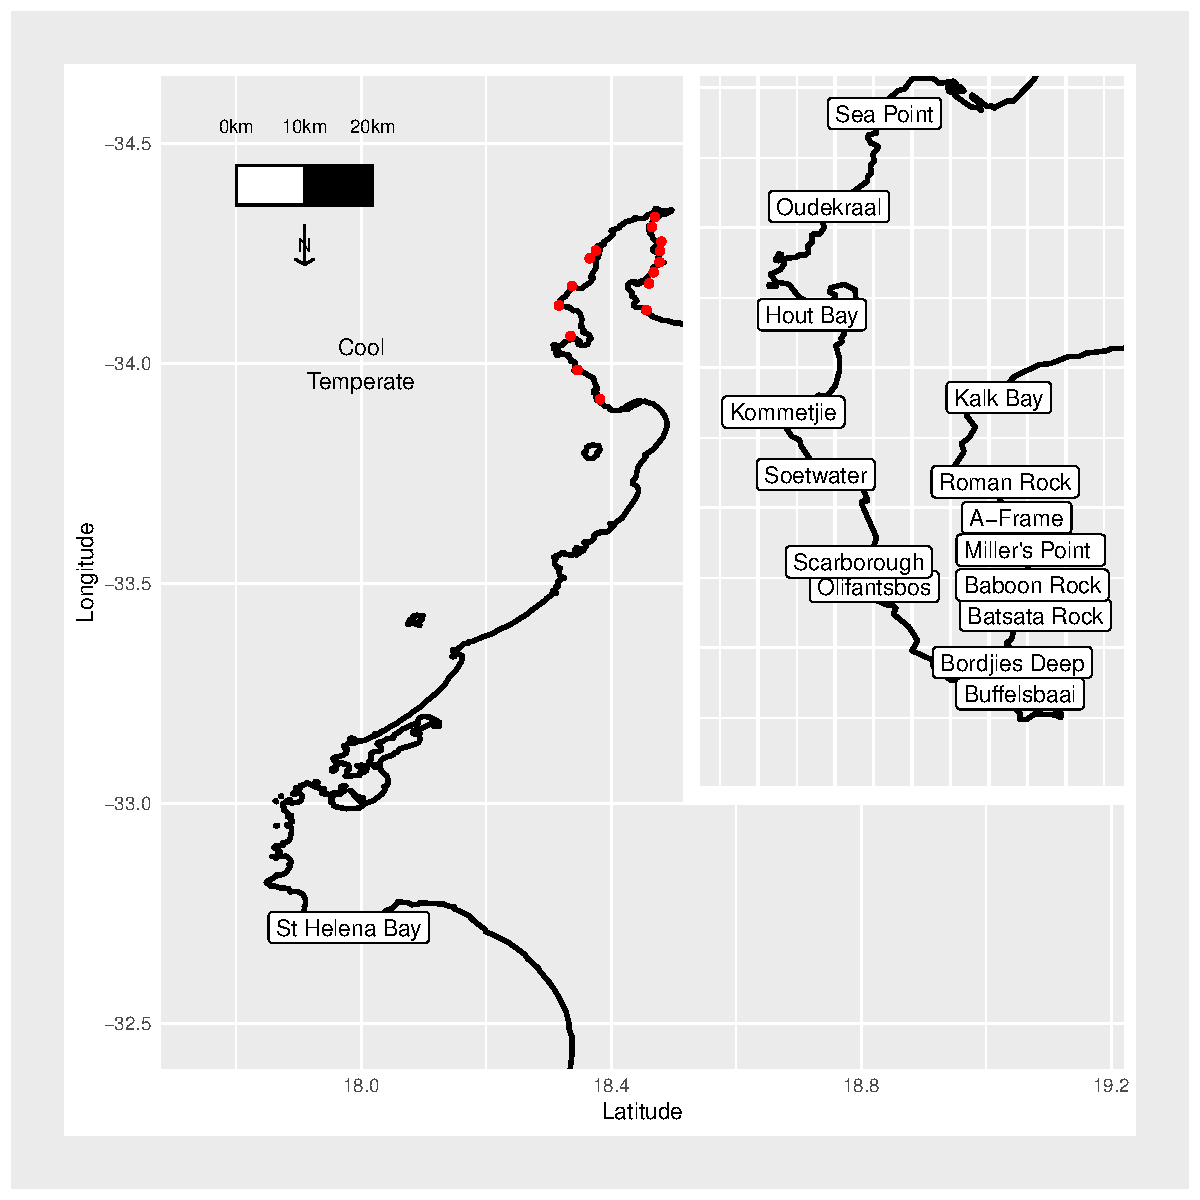
\includegraphics{thesis_chapter_2_files/figure-latex/map-1} 

}

\caption{\label{fig:map}Map of the study area and sampling sites. The red dot indicates the position of Cape Town for sake of reference.}\label{fig:map}
\end{figure}

The annual and seasonal patterns in both wind and swell direction
influence the thermal regime around the coastline by inducing upwelling.
Upwelling brings deep, cool nutrient-rich water to coastal areas which
causes a decrease in temperature (Field et al. 1980; Andrews and
Hutchings 1980; Gill and Clarke 1974; Cram 1970; Rouault, Pohl, and
Penven 2010; Blanke et al. 2002). The wind speed and wind direction help
drive upwelling in summer on the western side of the Cape Peninsula,
where southerly winds blow parallel to the coast and trigger upwelling
events (Field et al. 1980; Rouault, Pohl, and Penven 2010). This is not
the case for False Bay, which is shielded from the dominating wind and
swell that the Cape Peninsula is subjected to. In the summer months,
upwelling becomes more favorable in False Bay due to the change in swell
and wind direction, causing lower temperatures to dominate during this
time (Rouault, Pohl, and Penven 2010; Andrews and Hutchings 1980). Due
to the Cape Peninsula temperate latitude, winter months bring an
increased frequency of frontal depressions that originate from the
Southern Ocean (Reason, Landman, and Tennant 2006). These low pressures
are joined by large swells with increased wave energy. The nearshore
environment, with the accompanied biota, therefore experiences high wave
energy events, with increased frequency in winter (Veitch et al. 2019).
The large peninsula acts as an obstruction for large south westerly
swells, providing decreased wave energy along the west side of False Bay
(Shipley 1964). Conversely, the west coast of Cape Point is battered by
these large swells. Multiple sites, therefore, exist where kelps grow in
diverse temperature and wave energy climates, in close proximity and on
the same side. The topography and elevation along the Cape Peninsula
channel and shield winds along False Bay. This is, however, absent in
winter, when strong northerly winds are prevalent from St.~Helena Bay to
Betty's Bay (Field et al. 1980; Jury, Kamstra, and Taunton-Clark 1985;
Andrews and Hutchings 1980; Jury 1980).

\hypertarget{abiotic-environment}{%
\subsection{Abiotic environment}\label{abiotic-environment}}

In order to compare abiotic variables for sites around the coast, large
historical databases for temperature, wave energy and wind were
accessed.

\hypertarget{temperature}{%
\subsubsection{Temperature}\label{temperature}}

Shallow water temperatures were sourced from The South African Coastal
Temperature Network (SACTN) website1. In terms of nearshore temperature,
in situ data are preferred over satellite sea surface temperature (SST),
which have shown to exhibit large biases (Smit et al. 2013). The
underwater temperature recorders (UTRs) are attached to concrete mooring
blocks or railway line sections deployed in the shallow at ∼3 m depth.
The UTRs were comprised of Starmon Mini recorders (Star-Oddi, Reykjavik,
Iceland/Onset Hobo® U22-001) accurate to ±0.2°C. All in situ temperature
data were reduced to a time-coded, continuous series of monthly means
over various time-scales (Smit et al. 2013). It was decided that the
annual time-scale would be used for analysis. Linear interpolated SST
were calculated for sites where in situ recorders were absent. These
data were used to group sites into ``Cool temperate'' and ``Warm
temperate'' categorizations to investigate the possible effect of
thermal regime on kelp morphological characteristics.

\hypertarget{wave-environment}{%
\subsubsection{Wave environment}\label{wave-environment}}

Wave model variable data formed part of the South African Coastal
Vulnerability Assessment, presented to the Department of Environmental
Affairs (DEA) and produced by the Council for Scientific and Industrial
Research (CSIR) (Rautenbach 2015). The South African wave climate was
modeled via 20 spectral numerical wave models that simulated the
offshore wave climate to the nearshore. The boundary conditions of these
models were obtained by using the NOAA Wave Watch III (WWIII) model
output, distributed via the National Centers for Environmental
Prediction (NCEP) product (Office of the Director 2000; Environmental
Modeling Center/Marine Modeling Branch 2005). The particular hindcast
product utilized during the DEA-CSIR study spans 1994--2013 at a 3-hour
resolution. These data were then used to model swell propagation into
the coastal models while wind waves (seas) were generated via stationary
computations in the Simulating Waves in the Nearshore SWAN model (Booij,
Holthuijsen, and Ris 1997). The assumption of stationary computations is
acceptable as the model domains were small enough so the temporal
variation of the model boundary was slower than the time it takes for
that boundary condition to propagate to the coast. SWAN allows one to
extract wave variables from specific gridded locations in the nearshore.
For False Bay, a resolution of 200 meters was modeled and output
produced at both the 7 m and 15 m isobaths. A 200 m resolution was used
as the False Bay computational grid was nested within a larger 1 km
resolution grid. This allowed for a computational effective wave
resolution of increasing resolution, from the NCEP, low resolution
output to nested, high resolution coastal output. For Table Bay and east
of Cape Hangklip the resolution was 500 m and also had output at the 7
and 15 m isobaths. These contour outputs were chosen in the original
study by the CSIR as most engineering run-up calculations require wave
parameter information at these contour depths and were the main focus of
the original study. For this study the 7 m contours were used. These
data were then used to calculate over all wave power (kW/m) as this was
considered the best measure of overall wave exposure. Annual wave power
was plotted and categorized into different wave exposure categories
which ranged from fully sheltered to extremely exposed.

\hypertarget{collection-of-kelp-morphological-characteristics}{%
\subsubsection{Collection of kelp morphological
characteristics}\label{collection-of-kelp-morphological-characteristics}}

The morphological characteristics of both species are presented in
figure \ref{fig:schematic}. \emph{Laminaria pallida} is characterized by
a single smooth blade which is divided longitudinally into sections, and
develops from a single meristematic region located at the junction
between the blade and the stipe (Dyer 2018). This species has a solid
stipe along the south-west coast but develops a hollow stipe along the
west coast northward and into Namibia (Rothman et al. 2017).
\emph{Ecklonia maxima} consists of a single primary blade which develops
above a gas-filled float and a hollow stipe below. Secondary blades are
produced laterally from the primary blade from several meristematic
regions along the margins of the primary blade (Dyer 2018). Both species
are held to the substrate by finger-like haptera, collectively known as
the holdfast.

\begin{figure}

{\centering 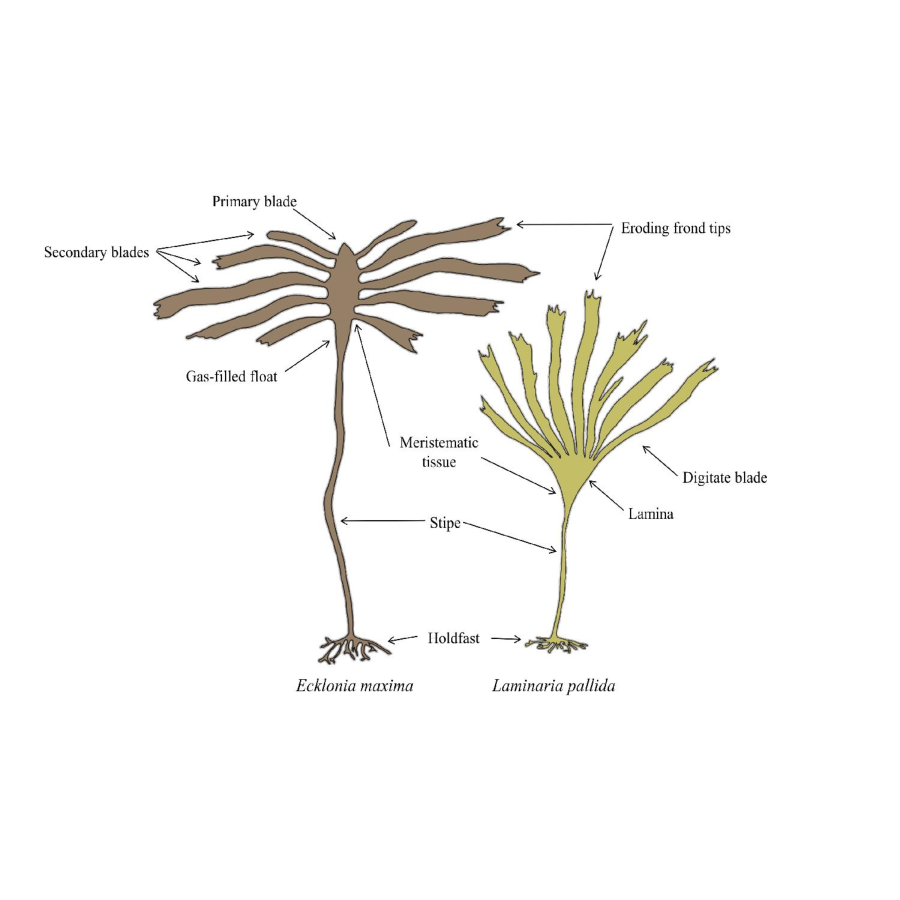
\includegraphics{thesis_chapter_2_files/figure-latex/schematic-1} 

}

\caption{\label{fig:schematic}Schematic of *Laminaria pallida* and *Ecklonia maxima* morphology [@Dyer2018-rv].}\label{fig:schematic}
\end{figure}

Morphological measurements of L. pallida and E. maxima were collected at
18 sites along the Western Cape coast of South Africa (Figure
\ref{fig:map}) between October 2014 and April 2015. AlgaeBase was used
to confirm the latest taxonomic associations for each species
({\textbf{???}}). Divers sampled kelp individuals by means of SCUBA for
deeper populations and freediving for shallower populations. The sampled
individuals were then taken ashore and the relevant morphological
measurements taken. In each instance only the 13 largest individuals
were sampled to ensure that only mature and fully grown sporophytes were
measured. The age of \emph{E. maxima} was determined by size, presence
at the surface as well as a darker coloration of the stipe; as this
occurs with age. In the case of \emph{L. pallida}, the individuals with
the longest stipe were selected which is considered a reasonable
estimate of age. In each case the age of the individuals was estimated
visually before the individual was sampled. In instances where one of
the species was not present a site, the nearest population of the
missing species was sampled. Because the macroalgae differ in
morphological features, species-specific morphological characteristics
were included and are presented in Table 1. The stipe length for
\emph{E. maxima} was considered to be the portion of the plant just
below the pneumatocyst and just above the holdfast. Stipe circumference
was measured just above the holdfast for both species. Between February
2017 and November 2018, morphological measurements for E. maxima
individuals in shallow water (\textless1 m) at seven sites along the
Western Cape coast of South Africa were also collected. The same
morphological characteristic measurements were taken as for the deeper
\emph{E. maxima}, and this allowed comparison between morphological
characteristics between deep and shallow individuals within sites.
Measurements were not collected for \emph{L. pallida} in the shallow
depths, as this species is largely absent from the shallow in this
portion of the South African coastline.

\hypertarget{statistical-analyses}{%
\subsection{Statistical analyses}\label{statistical-analyses}}

Summary statistics were calculated for each site and region for each of
the environmental variables considered in this study, and are presented
in Table 2. The associated abbreviations used are also presented in
Table 2. In addition, annual median wave and wind direction were also
calculated. The median was calculated for wind and wave direction, as
issues arise when calculating the mean and standard deviation for
compass metrics. Summary statistics for wind was not plotted and instead
are discussed, as the data were course relative to the other
environmental variables considered in this study.

Morphological characteristics in relation to temperature and wave
exposure were investigated using non-parametric statistical methods.
Morphological characteristics were placed into categories according to
temperature regime and wave exposure class for each species and
population of kelp in this study. The appropriate category was
determined by kelp's sampling location along the coastline and the
according wave exposure and temperature category assigned to that
species and/or population. The R software package ggplot2 was used for
graphical output and non-parametric analyses. Significant differences
between temperature regimes and across wave exposure categories were
tested with Wilcox tests and Kruskal -Wallis tests, respectively, and
notched boxplots allowed comparison between individual categories of
wave exposure. The alpha level used to define significance was p = 0.05.
Boxplots were created using the software package ggplot2
({\textbf{???}}). In order to investigate specific drivers of
morphological characteristics a distance-based redundancy analysis
(db-RDA) was performed using the rda function in the vegan software
package (Oksanen et al. 2015) in R (R Core Team, 2014; RStudio Team,
2020). The abiotic data covered all study sites for both species of
kelp. Both morphology and abiotic data (temperature, waves and wind)
were standardized using the decostand function in the vegan software
package; morphology data were used as response variables and the abiotic
data as explanatory variables. A list of the abbreviations used and the
associated metrics are presented in Table 2. To determine the
explanatory variables that best describe patterns in the response data,
a full RDA was performed using a complete set of explanatory variables.
Forward selection was then used to reduce the number of explanatory
variables, as well as prevent the inflation of overall Type I error. To
further improve the model, pairwise coefficients and Variance Inflation
Factor (VIF) were calculated to identify variables with high
multicollinearity. The computation of the parsimonious RDA was followed
by permutation tests of the adjusted R2 to assess significance of
constraints.

\hypertarget{results}{%
\section{Results}\label{results}}

\hypertarget{abiotic-environment-1}{%
\subsection{Abiotic environment}\label{abiotic-environment-1}}

\hypertarget{temperature-1}{%
\subsubsection{Temperature}\label{temperature-1}}

The mean annual coastal water temperature for the study sites located on
the western side of the peninsula ranged from 14.5 ± 0.9°C (mean ± SD)
at St.~Helena Bay, the most northern site on the western side of the
peninsula, to 14.6 ± 0.3°C at Olifantsbos, the most southern site on the
western side of the peninsula (see Figure
\ref{fig:Temperature variables plot}A). For sites located on the eastern
side of the peninsula (within False Bay), the annual mean coastal water
temperatures ranged from 15.5 ± 0.9°C at Buffelsbaai to 15.0 ± 0.9°C at
Betty's Bay, the most eastern site on the coastline in this study (see
Figure \ref{fig:Temperature variables plot}A).

\begin{figure}

{\centering 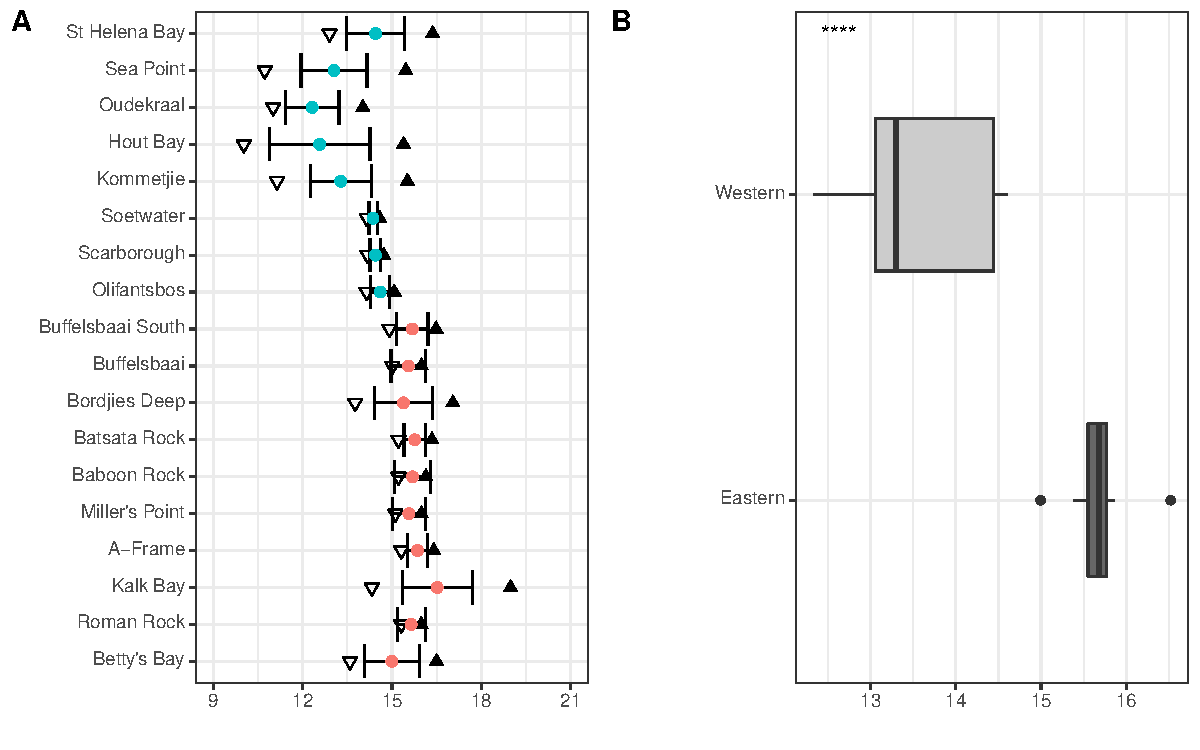
\includegraphics{thesis_chapter_2_files/figure-latex/Temperature variables plot-1} 

}

\caption{\label{fig:Temperature variables plot}Annual temperature variables at the collections sites around the Cape Peninsula are represented by plot A, with sites in order from North to South. Temperature variables include minimum temperature represented by inverted triangles, mean represented by black dots, maximum by black triangles, and whiskers standard deviation. Summary of temperature data for sites grouped by region and represented in plot B.}\label{fig:Temperature variables plot}
\end{figure}

In general, the mean temperature increases for sites located within
False Bay with less variation around the mean temperature compared to
sites on the western side of the peninsula (see Figure
\ref{fig:Temperature variables plot}A). This is verified by statistical
difference based on region, which shows a significantly lower (p
\textless{} 0.05, Figure \ref{fig:Temperature variables plot}B) mean
temperature and less variation in temperature for sites located on the
western side of the peninsula compared to sites on the eastern side.

\hypertarget{wave-environment-1}{%
\subsubsection{Wave environment}\label{wave-environment-1}}

Our data show the western side of the peninsula experiences higher
significant wave heights and variation in wave heights compared to the
eastern side of the peninsula (see Figure
\ref{fig:wave variable plot})A). Mean significant wave height ranged
from 0.5 ± 0.2 m (mean ± SD) at St.~Helena Bay to 2.3 ± 0.7 m at
Olifantsbos on the western side of the peninsula, and on the eastern
side of the peninsula it ranged from 0.9 ± 0.4 m at Buffelsbaai to 1.9 ±
0.6 m at Betty's Bay (see Figure \ref{fig:wave variable plot})A). The
maximum significant wave height ranged from 1.4 m at St.~Helena Bay to
4.7 m at Olifantsbos on the western side of the peninsula, and on the
eastern side ranged from 2.6 m at Buffelsbaai to 4.2 m at Betty's Bay.
Mean peak period for sites on the western side of the peninsula ranged
from 10.3 ± 3.5 s at St.~Helena Bay to 11.0 ± 2.0 s at Olifantsbos, and
ranged from 10.6 ± 3.0 s at Buffelsbaai to 10.8 ± 2.2 s at Betty's Bay
(see Figure \ref{fig:wave variable plot})B). The data show no trend in
mean peak period for the coastline. These data show that the western
side of the peninsula has a lower variation (SD) compared to the eastern
side, with Miller's Point showing the highest variation across
timescales. Maximum peak period ranged from 18.9 s at St.~Helena Bay to
18.4 s at Olifantsbos for the western side of the peninsula, and ranged
from 18.0 s at Buffelsbaai to 18.0 s at Betty's Bay on the eastern side
of the peninsula. When wave variables were grouped by region significant
differences were found for both mean significant swell height and mean
peak period. The western region experiences a significantly higher mean
significant swell height (p \textless{} 0.05; see Figure
\ref{fig:wave variable plot})C) and mean peak period (p \textless{}
0.05; see Figure \ref{fig:wave variable plot})D).

Data for median wave direction showed no trend across timescales,
however, the variation (SD) in wave direction is lower on the western
side of the peninsula compared to the eastern side both annually and for
winter. Summer data were the exception and showed lower variation for
the eastern side of the peninsula (see Appendix).

In Figure 5A the total coastal wave exposure of the Cape Peninsula is
given in terms of wave energy (kW per meter wave crest length). The
classification from fully sheltered to extremely exposed is based on the
total wave energy upper and lower limits (see Figure
\ref{fig:wave power map}B). The western periphery of the Cape Peninsula
is almost continuously exposed to high wave exposures while the eastern
periphery of the peninsula (western coastline of False Bay) revealed
sheltered wave exposures (see Figure \ref{fig:wave power map}). There
the marked seasonality, with higher energy waves during winter, may be
clearly observed once more.

\begin{figure}

{\centering 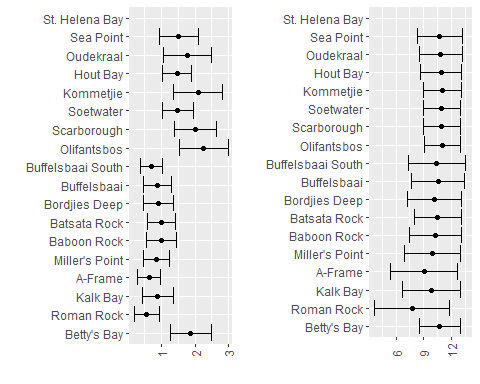
\includegraphics{thesis_chapter_2_files/figure-latex/wave variable plot-1} 

}

\caption{\label{fig:wave variable plot}Mean significant wave height and mean significant peak period across sites and by region. Mean significant wave height across sites is presented in plot A and is represented by solid triangles and standard deviation by the whiskers. Differences in mean significant wave height between regions are presented in plot B. Mean significant peak period across sites is presented in plot C and is represented by solid dots and standard deviation by whiskers. Differences in mean significant peak period between regions are presented in plot D.}\label{fig:wave variable plot}
\end{figure}

\begin{figure}

{\centering 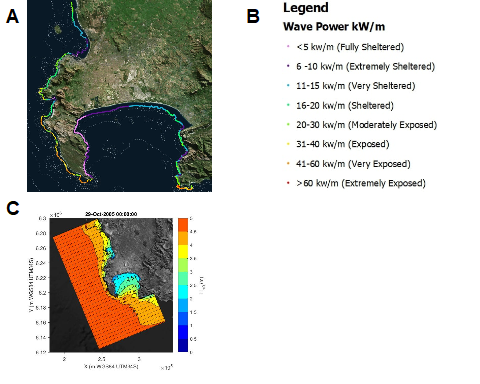
\includegraphics{thesis_chapter_2_files/figure-latex/wave rose-1} 

}

\caption{\label{fig:wave rose}The total and seasonal wave roses of the directional wave buoy just offshore from Cape Town is given form the years 2000 till end 2017 (the period for which directional wave spectra was available). Total (A), Austral winter (B) and Austral summer (C) respectively}\label{fig:wave rose}
\end{figure}

\begin{figure}

{\centering 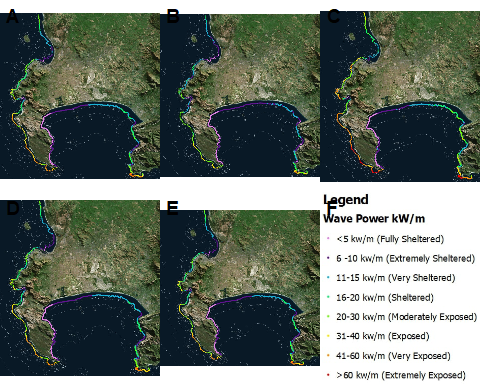
\includegraphics{thesis_chapter_2_files/figure-latex/wave power map-1} 

}

\caption{\label{fig:wave power map}The total coastal wave exposure of the Cape Peninsula is given in terms of wave energy (kW per meter wave crest length. Total (A), summer (B), winter (C), spring (D) and autumn (E).}\label{fig:wave power map}
\end{figure}

To clarify the averaged wave exposure map presented in Figure
\ref{fig:wave power map}A, the propagation of a typical offshore wave
spectrum as produced from a single time-step in SWAN is presented in
Figure \ref{fig:wave power map}C. Tracing the wave height contours into
False Bay its clear why this bay's western periphery is predominantly
sheltered.

\begin{figure}

{\centering 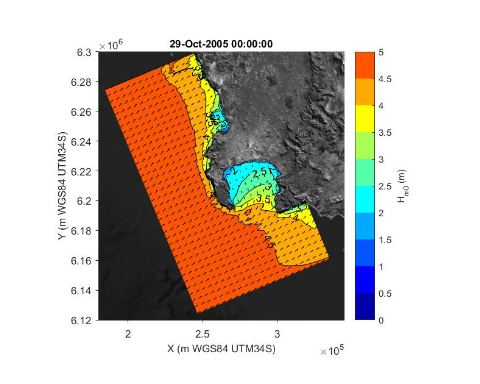
\includegraphics{thesis_chapter_2_files/figure-latex/FB spectrum-1} 

}

\caption{\label{fig:FB spectrum}The propagation of a typical offshore wave spectrum is given as produced from a single time-step in SWAN.}\label{fig:FB spectrum}
\end{figure}

\hypertarget{drivers-of-kelp-morphological-characteristics}{%
\subsection{Drivers of kelp morphological
characteristics}\label{drivers-of-kelp-morphological-characteristics}}

Significant differences were found between cool temperate and warm
temperate regimes for most \emph{L. pallida} morphological
characteristics with lamina length, number of digits and thallus mass
the exceptions (see Figure 6). Certain morphological characteristics
such as stipe mass, stipe length, total length and stipe diameter had
significantly higher means for kelp from the cool temperate regime when
compared to kelp from the warm temperate regime (p \textless{} 0.05; see
Figure \ref{fig:lamanaria temp plots}). Conversely, lamina weight and
lamina thickness had significantly lower means for kelp from the cool
temperate regime compared to kelp from the warm temperate regime. When
\emph{L. pallida} morphological characteristics were grouped to wave
exposure categories Kruskal-Wallis tests revealed significant
differences amongst categories for most morphological characteristics
with lamina length, number of digits and thallus mass the exceptions
(see Figure ref\{fig:lamanaria wave plots\}). The morphological
characteristics that were significantly different amongst sites
exhibited similar patterns, with increasing mean values from the fully
sheltered to extremely sheltered categories and a decrease in mean
values for the remainder of the categories. Two morphological
characteristics, namely lamina thickness and stipe diameter, both
exhibited higher variations for the exposed categories compared to other
morphological characteristics.

\begin{figure}

{\centering 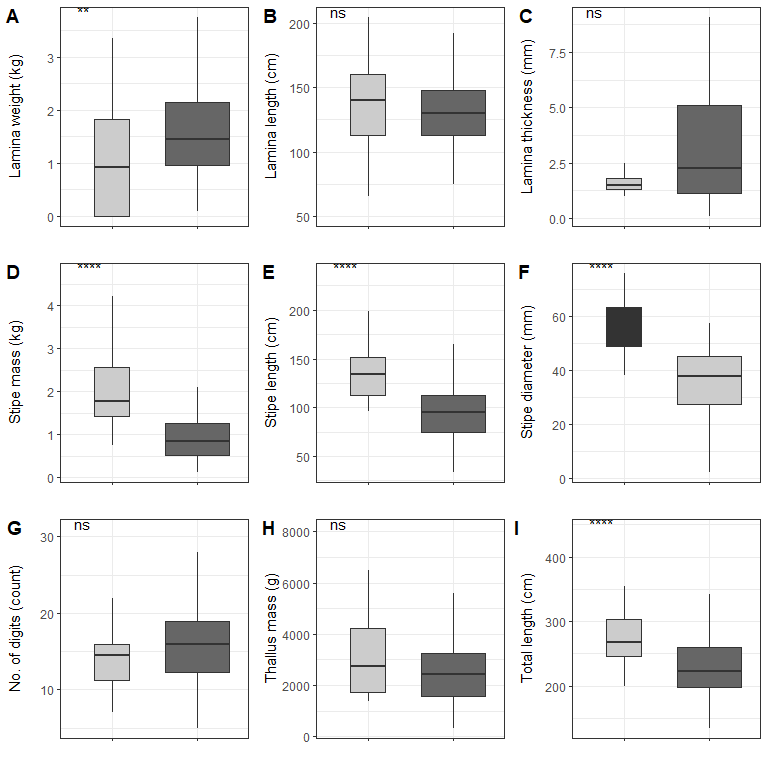
\includegraphics{thesis_chapter_2_files/figure-latex/laminaria temp plots-1} 

}

\caption{\label{fig:lamanaria temp plots}Boxplots representing *L. pallida* morphological characteristics grouped by temperature regime measured around the Western Cape coastline, with the *y*-axis depicting the specific morphology measured, with units provided. The lower and upper "hinges" correspond to the first and third quartiles. The whiskers represent the range, solid black lines represent the median and black dots are outliers. Light grey boxes represent cool-temperate and dark grey warm-temperate.}\label{fig:laminaria temp plots}
\end{figure}

\begin{figure}

{\centering 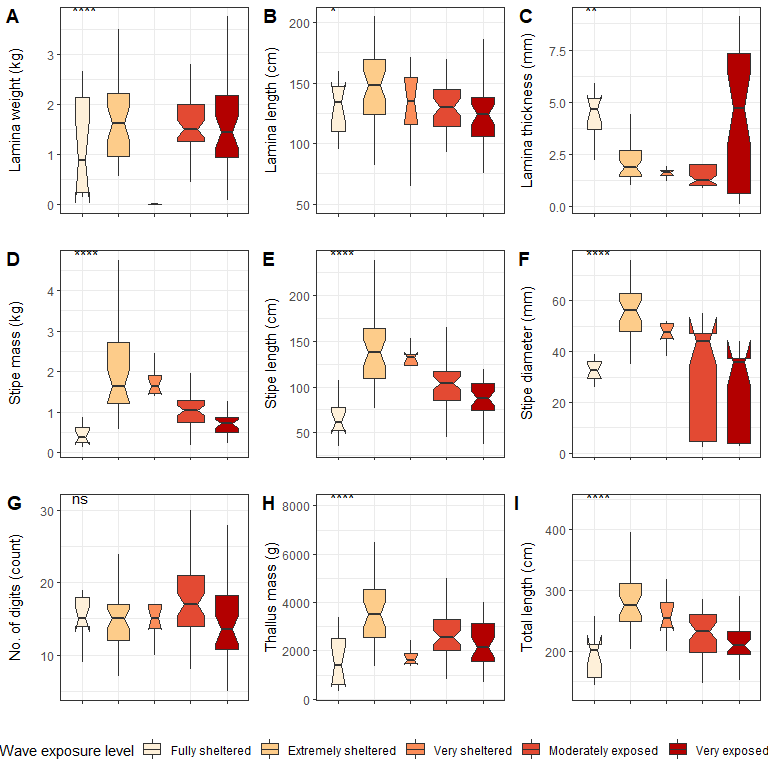
\includegraphics{thesis_chapter_2_files/figure-latex/lamanaria wave plots-1} 

}

\caption{\label{fig:lamanaria wave plots}Boxplots representing *L. pallida* morphological characteristics grouped by wave exposure category measured around the Western Cape coastline, with the *y*-axis depicting the specific morphology measured, with units provided. The lower and upper hinges correspond to the first and third quartiles. The whiskers represent the range, solid black lines represent the median and black dots are outliers.}\label{fig:lamanaria wave plots}
\end{figure}

Six out of the ten deep \emph{E. maxima} morphological characteristics
showed differences between cool temperate and warm temperate regime
except for frond mass, frond length, stipe mass and epiphyte length.
Mean values for primary length, primary width and stipe circumference
were significantly higher for kelp from the cool temperate regime than
for kelp from the warm temperate regime (see Figure
\ref{fig:{deep eck temp plot}}). The remaining morphological
characteristics, stipe length, number of tufts and total length had
significantly lower means for kelp from cool temperate compared to kelp
from the warm temperate regime (p \textless{} 0.05; see Figure 8).
Significant differences amongst wave exposure categories were found for
all morphological characteristics of deep E. maxima populations (see
Figure \ref{fig:deep eck temp plot} ). Certain morphological
characteristics showed a gradual increase in mean value with increasing
degree of wave exposure. The remaining morphological characteristics
exhibited decreased means for only the higher wave exposure categories,
followed by a sharp increase in mean value for the highest wave exposure
category.

\begin{figure}

{\centering 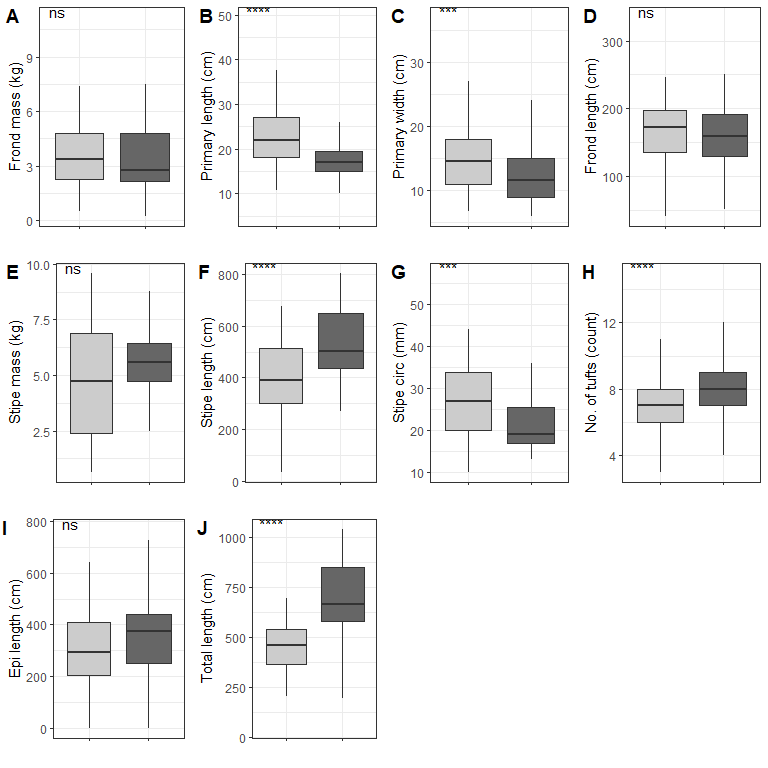
\includegraphics{thesis_chapter_2_files/figure-latex/deep ecklonia temp plot-1} 

}

\caption{\label{fig:deep eck temp plot}Boxplots representing deep population *E. maxima* morphological characteristics grouped by temperature regime measured around the Western Cape coastline, with the *y*-axis depicting the specific morphology measured, with units provided. The lower and upper hinges correspond to the first and third quartiles. The whiskers represent the range, solid black lines represent the median and black dots are outliers. Light grey boxes represent cool-temperate and dark grey warm-temperate.}\label{fig:deep ecklonia temp plot}
\end{figure}

\begin{figure}

{\centering 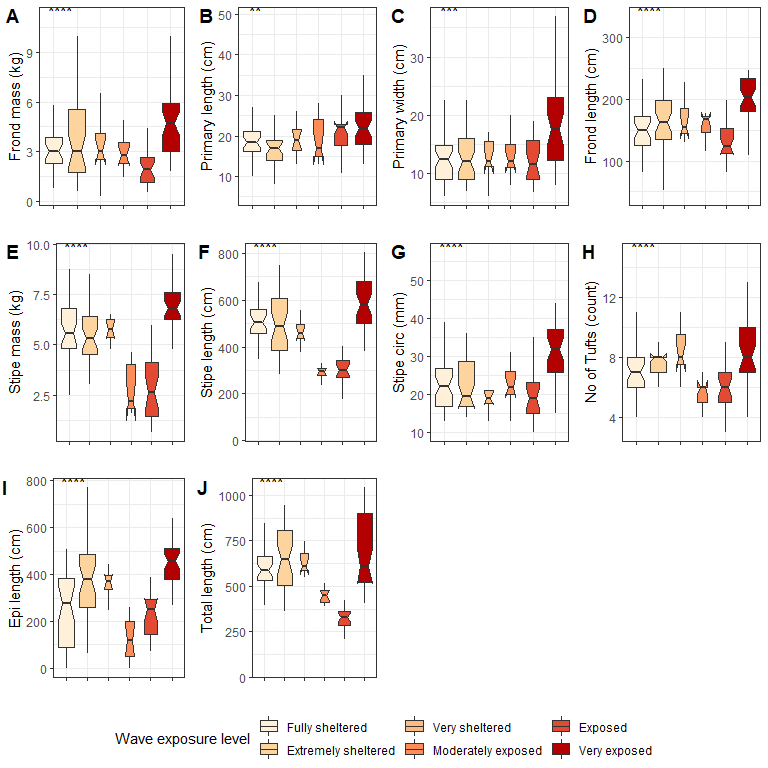
\includegraphics{thesis_chapter_2_files/figure-latex/deep ecklonia wave-1} 

}

\caption{\label{fig:deep ecklonia wave}Boxplots representing deep *E. maxima* morphological characteristics grouped by wave exposure category measured around the Western Cape coastline, with the *y*-axis depicting the specific morphology measured, with units provided. The lower and upper hinges correspond to the first and third quartiles. The whiskers represent the range, solid black lines represent the median and black dots are outliers.}\label{fig:deep ecklonia wave}
\end{figure}

\begin{figure}

{\centering 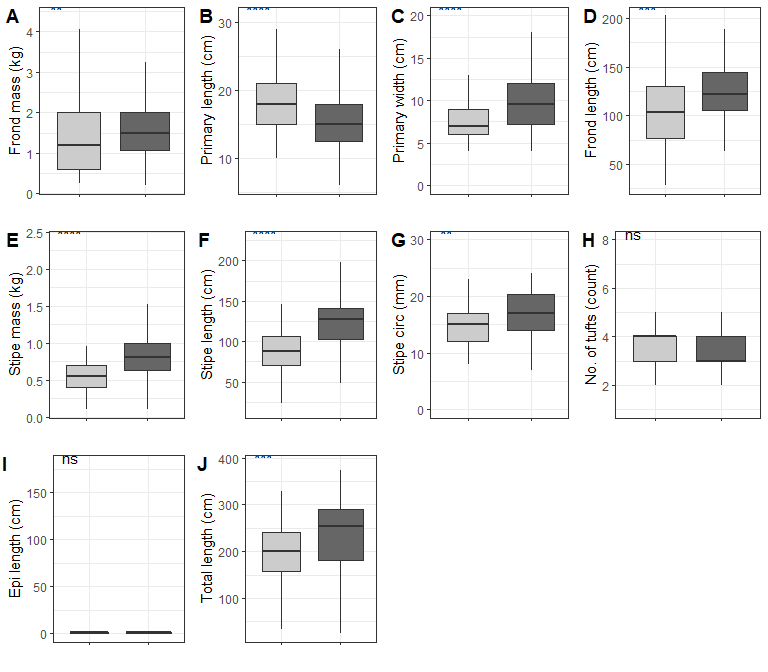
\includegraphics{thesis_chapter_2_files/figure-latex/shallow ecklonia temp-1} 

}

\caption{\label{fig:shallow ecklonia temp} Boxplots representing shallow *E. maxima* morphological characteristics  grouped by temperature regime measured around the Western Cape coastline, with the *y*-axis depicting the specific morphology measured, with units provided. The lower and upper hinges correspond to the first and third quartiles. The whiskers represent the range, solid black lines represent the median and black dots are outliers. Light grey boxes represent cool-temperate and dark grey warm-temperate.}\label{fig:shallow ecklonia temp}
\end{figure}

\begin{figure}

{\centering 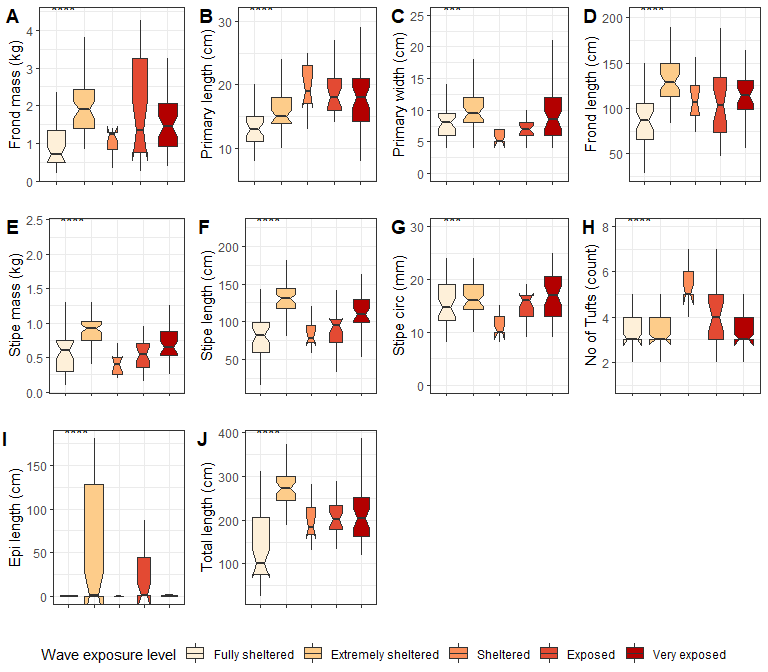
\includegraphics{thesis_chapter_2_files/figure-latex/shallow ecklonia wave-1} 

}

\caption{\label{fig:shallow ecklonia wave}Boxplots representing shallow *E. maxima* morphological characteristics grouped by wave exposure category measured around the Western Cape coastline, with the *y*-axis depicting the specific morphology measured, with units provided. The lower and upper hinges correspond to the first and third quartiles. The whiskers represent the range, solid black lines represent the median and black dots are outliers.}\label{fig:shallow ecklonia wave}
\end{figure}

When grouped by temperature regime, shallow \emph{E. maxima} exhibited
significant differences between temperature regimes for frond mass,
primary length, primary width, frond length, stipe mass, stipe length,
stipe circumference and total length (p \textless{} 0.05; see Figure
\ref{fig:shallow ecklonia temp}). All of the significantly different
morphological characteristics, except primary length, had lower values
for the western region compared to the eastern region. When shallow E.
maxima were grouped by wave exposure category significant difference
were found for all morphological characteristics (p \textless{} 0.05;
see Figure \ref{fig:shallow ecklonia wave}). In general, values of the
various morphological characteristics increase for the lower wave
exposure categories, followed by a sharp decrease and a gradual increase
in value.

\hypertarget{abiotic-drivers-of-l.-pallida-morphological-characteristics}{%
\subsubsection{\texorpdfstring{Abiotic drivers of \emph{L. pallida}
morphological
characteristics}{Abiotic drivers of L. pallida morphological characteristics}}\label{abiotic-drivers-of-l.-pallida-morphological-characteristics}}

Forward selection, assessment of VIF and an examination of pairwise
Pearson correlation coefficients allowed us to retain the most
parsimonious descriptors of L. pallida morphological characteristics
with an adjusted R2 of 0.49, explaining 72\% of the variation (global
permutation test on final model: d.f = 1, F = 8.51, p = 0.008; Figure
\ref{fig:rda plots}A). RDA1 was the only significant axis in the model
and explained 48\% of the variation while RDA2 was not significant and
explained 63\% of the variation. Total length, stipe length, stipe
diameter and stipe mass were positively influenced (i.e., increased size
corresponding with the environmental driver) by mean significant wave
height and median swell direction for kelp mostly from the western
region and negatively influenced (i.e., decreased size corresponding
with the environmental driver) by peak period standard deviation and
mean temperature for kelp from the eastern region. Although sites from
the western region did not cluster as closely as eastern region study
sites, grouping according to region was still evident.

\hypertarget{abiotic-drivers-of-e.-maxima-morphological-characteristics}{%
\subsubsection{\texorpdfstring{Abiotic drivers of \emph{E. maxima}
morphological
characteristics}{Abiotic drivers of E. maxima morphological characteristics}}\label{abiotic-drivers-of-e.-maxima-morphological-characteristics}}

The same approaches to identify the descriptors for \emph{L. pallida}
were employed for both populations of \emph{E. maxima}. Forward
selection, assessment of VIF and Pearson correlation coefficients
allowed us to retained as the most parsimonious descriptors of deep
\emph{E. maxima} morphological characteristics with an adjusted R2 of
0.39, explaining 67\% of the variation (global permutation test on final
model: d.f = 5, F = 2.4, p = 0.026; Figure \ref{fig:rda plots}B). RDA1
was the only significant axis in the model (p = 0.03) and explained 72\%
of the variation. Primary length, primary width and stipe circumference
were positively influenced by mean significant wave height, mean peak
period and median swell direction for kelp from the western region. The
remaining morphological characteristics were positively influenced by
minimum temperature and negatively influenced by peak period standard
deviation for kelp from the eastern region.

\begin{figure}

{\centering \includegraphics{thesis_chapter_2_files/figure-latex/rda plots-1} 

}

\caption{\label{fig:rda plots}RDA output for *L. pallida* (A), deep *E. maxima* (B) and shallow *E. maxima* (C). The blue cluster represnts sites from the western region and the red represents sites from the eastern region.}\label{fig:rda plots}
\end{figure}

Forward selection, assessment of VIF and Pearson correlation
coefficients allowed us to retain the most parsimonious descriptors of
shallow \emph{E. maxima} morphological characteristics with an adjusted
R2 of 0.36, explaining 61\% of the variation (global permutation test on
final model: d.f = 4, F = 2.41, p = 0.013, Figure \ref{fig:rda plots}C).
The model consisted of one significant axis, RDA1 (p = 0.02) and
explained 62\% of the variation. Stipe length, stipe mass and stipe
circumference were positively influenced by maximum temperature and mean
temperature along RDA1, and explained 50 and 55\% of the variation,
respectively. The remaining morphological characteristics were
positively influenced by maximum peak period and negatively influenced
by median wind direction along RDA2 and explained 86 and 94\% of the
variation, respectively. There was overlapping of clusters according to
region with no clear patterns in sites evident.

\hypertarget{discussion}{%
\section{Discussion}\label{discussion}}

This study considered important drivers of the morphology of Ecklonia
maxima and Laminaria pallida around the Cape Peninsula. These abiotic
variables, namely temperature and wave exposure, have been identified in
previous research on other brown algae species such as E. radiata and M.
pyrifera (Thomsen, Wernberg, and Kendrick 2004; Fowler-Walker, Connell,
and Gillanders 2005; Fowler-Walker, Wernberg, and Connell 2006; Wernberg
and Thomsen 2005; Wing et al. 2007; Stewart et al. 2009; Miller, Hurd,
and Wing 2011; Pedersen and Nejrup 2012). The complex geomorphology of
the Western Cape coastline creates an ideal natural laboratory for
studies of kelps in interaction with their environment. Unlike previous
research, this study used a complex numerical model to provide the
various variables of wave exposure, which is based on linear wave theory
to calculate overall wave exposure. We also considered wind in addition
to temperature and wave variables, since wind is an important component
of wind-driven surface gravity waves (Holthuijsen 2010). The results
show that specific variables of wave exposure are the main drivers of
kelp morphology with temperature playing only a minor role. The
morphological adaptation was also shown to be associated with the
magnitude of wave exposure which had only been inferred in previous
studies. Finally, the investigation of differences in morphological
characteristics between shallow and deep populations of E. maxima
suggests that in low wave exposure environments the role of temperature
as a morphological driver increases; this is particularly the case for
False Bay.

There were clear patterns and clines in both the temperature and wave
exposure data. The thermal and wave exposure regimes around the Cape
Peninsula are driven by a complex interaction between wind, temperature
and wave metrics, which do not act independently but instead influence
one another. The hydrodynamic regime is modulated by the relative
sheltering against the predominant south-westerly swell direction and
the size of the fetch for local wave generation. The direction of the
dominant swell changes to the south west in winter, generated by strong
low pressures that originate from the southern ocean (Reason, Landman,
and Tennant 2006), which False Bay is sheltered from (Shipley 1964;
Atkins 1970; Dufois and Rouault 2012). In summer, these swells rotate
anticlockwise and are able to enter False Bay, providing an increased
variability of swell height and peak period in this region. It should be
noted that what is classified as sheltered around the South African
coastline (a high energy coastline) might be classified as exposed in
other regions of the world (Norderhaug et al. 2012; Leliaert et al.
2000). It is due to the near consistent south-westerly swell and the
complex orography around the peninsula that the wave energy distribution
around the Cape Peninsula varies significantly over a small geographical
area. The directional sheltering effect of the Cape Peninsula, against
the dominant swell direction is clearly observed in the wave exposure
maps. It should be mentioned that some of the annual winter frontal
depression systems pass the Cape Peninsula from the west to east,
resulting in wave propagating toward the continent from much more
southerly directions. This results in positive and negative wave
exposure anomalies all around the peninsula. Increased wind speed at
sites along the west side of the peninsula in a southerly direction
trigger upwelling events along the western side of the peninsula
(Rouault, Pohl, and Penven 2010; Field et al. 1980). In general, the
western side of the peninsula is more exposed than the eastern side
(False Bay) and experiences significantly higher mean significant swell
height and mean significant peak period. This was also reflected in the
wave exposure categories which show a trend of decreasing wave exposure
(wave power) around the peninsula and into False Bay. There are also
differences between the types of waves that each side of the peninsula
experiences. We provide strong support that variations in the
environmental variables, particularly wave exposure variables, are
driving kelp morphological characteristics around the Cape Peninsula.
Morphological adaptation due to water motion may manifest in a number of
ways in high wave energy environments. For instance, reduction of blade
thickness, blade elongation, increase of stipe length, increase in stipe
circumference and force of attachment (Fowler-Walker, Wernberg, and
Connell 2006; Wernberg and Thomsen 2005; Friedland and Denny 1995; Denny
and Gaylord 2002; Bekkby et al., n.d.; Denny, Gaylord, and Cowen 1997)
have been identified in previous studies. Although this study did not
measure force of attachment, other morphological responses to
temperature and wave variables were evident. Species-specific responses
are evident in both wave exposure and temperature. In cool temperate
environments \emph{L. pallida} tended to show increases in certain
morphological characteristics (stipe mass, stipe length and stipe
diameter) while in the warm-temperate environments these were
significantly lower. This was also true for deep \emph{E. maxima}
populations, which had longer, thinner stipes for kelp from the warm
temperate compared to kelp from the cool temperate. Reduction in certain
morphological characteristics has been attributed to temperature by
Serisawa et al. (2002) in the kelp E. cava, which was smaller and
shorter in warmer sites compared to cooler sites. The reduction in size
of adult may be a response to low nutrient conditions, which has been
shown to reduce growth rate and overall morphology (Simonson,
Scheibling, and Metaxas 2015). Warmer temperatures are associated with
low nutrient concentrations (Waldron and Probyn 1992) and the low
frequency of upwelling conditions in False Bay (low nutrient supply)
coupled with warmer temperatures may be a contributing factor. It should
be noted, however, that from these analyses that in general the cool
temperate region is more exposed to waves than that of the
warm-temperate region. Therefore, the significantly larger morphological
characteristics for kelp from the cool temperate region may overlap with
responses to wave exposure. The response of kelp morphological
characteristics to wave exposure was evident and both species exhibit
tactics based on the magnitude of wave exposure. Strength increasing
traits were exhibited for lower exposure levels while a
``go-with-the-flow'' tactic for moderate levels of wave exposure. This
suggests that how morphological characteristics manifest themselves is
dependent on the magnitude of wave exposure. When grouped by wave
exposure category, \emph{L. pallida} characteristics showed a
significant increase in length for the ``extremely sheltered'' category
compared to the fully sheltered category, which may be a
``go-with-the-flow'' tactic (Denny, Gaylord, and Cowen 1997; Denny and
Gaylord 2002; Hurd 2000). Kelp are able to increase flexibility by
increasing stipe length which increases the extension capabilities of
kelp to a passing wave (Denny, Gaylord, and Cowen 1997; Denny and
Gaylord 2002; Hurd 2000). However, increasing stipe length is only
beneficial under lower exposure levels as a long stipe actually
increases overall drag on the plant under high wave exposure (Denny,
Gaylord, and Cowen 1997; Denny and Gaylord 2002; Hurd 2000). This is
reflected in the \emph{L. pallida} morphology which shows an overall
reduction of morphological characteristics suggesting a size reducing
tactic to cope with higher levels of wave exposure. The results suggest
that deep \emph{E. maxima} populations exhibit a different response, as
well as a higher wave exposure threshold. Unlike \emph{L. pallida},
\emph{E. maxima} exhibits a size reducing tactic with increasing wave
exposure by decreasing stipe mass, stipe length, stipe circumference,
total length and frond length. A magnitude related response has been
suggested by Wernberg and Vanderklift (2010) who investigated the
temporal and spatial variations of various environmental drivers of the
kelp \emph{E. radiata}. The authors identified wave exposure as the most
important driver of kelp morphological characteristics and that the type
of response elicited is dependent on the magnitude of wave exposure.

A size reduction tactic has been shown before (Fowler-Walker, Wernberg,
and Connell 2006; Denny and Gaylord 2002; Hurd 2000; Fowler-Walker,
Connell, and Gillanders 2005) and is regarded as a strategy to reduce
overall drag on the plant. However, \emph{E. maxima} morphological
characteristics changed significantly as wave exposure increases. When
grouped to the higher wave exposure levels, \emph{E. maxima} morphology
exhibited a strength and flexibility increasing trait. Furthermore, the
morphological response of \emph{E. maxima} to wave exposure only occurs
at the ``Moderately exposed'' level compared to \emph{L. pallida} which
exhibits a response at a lower wave exposure level. This suggests that
\emph{E. maxima} can tolerate higher exposure levels before having to
exhibit a morphological response. The redundancy analysis performed
confirms the patterns and responses observed as well as identifying
specific temperature and wave variables as drivers of kelp morphology.
Kelp morphology characteristics are largely wave driven for both species
but differ in terms of specific temperature and wave metrics.

The wave metrics identified in this study are important components of
determining overall wave power, which will vary seasonally in the region
based on the swell direction. The differences in temperature metrics
between \emph{E. maxima} and \emph{L. pallida} point to underlying
differences in nutrient availability. Low temperatures are often
associated with upwelling events which bring cool, nutrient rich water
into the nearshore. False Bay has comparatively little upwelling events
compared to the western side of the peninsula, and so nutrients may be a
limiting factor for \emph{E. maxima} populations within False Bay, hence
the identification of minimum temperature as a influencer. Mean
temperature identified as a driver for \emph{L. pallida} may be related
to diurnal temperature fluctuations in the water column. Solar heating
of the water surface in combination with wind-driven transport causes
fluctuations within the water column, which can occur daily or
seasonally (Kaplan et al. 2003). Vertical mixing of the water column for
inshore regions are driven by several abiotic processes: (1) turbulence
of breaking waves inside or outside of the surf zone; (2) convective
mixing through a combination of cooling and evaporation; (3) wind driven
currents; and (4) tidal mixing (Smit et al. 2013). These abiotic
processes cause effective vertical mixing of surface and deeper water
stratification which leads to a homogeneous thermal environment, which
in this study may be interpreted as the mean temperature. Therefore, the
homogeneous thermal regime of inshore regions may be a reason why mean
temperature is driver of \emph{L. pallida} morphological
characteristics. The difference in canopy type between the species may
be the reason why \emph{E. maxima} is driven by multiple wave metrics
compared to \emph{L. pallida}. Since \emph{E. maxima} are a canopy-kelp,
it is exposed to all components of a wave compared to \emph{L. pallida}
which occurs deeper in the water column.

Although temperature plays an important role in distribution (Bolton
2010; Miller, Hurd, and Wing 2011; Rinde et al. 2014) of kelp and
physiological functioning of adults and gametophytes (Mohring et al.
2014; Steneck et al. 2002; Gerard 1997; Bearham, Vanderklift, and Gunson
2013; Smale and Moore 2017), there is little evidence in this study that
temperature is an important driver of morphological variation. However,
we suggest that temperature plays a larger role in determining kelp
morphology at sites where wave energy is low enough not to elicit a
response in morphological characteristics. Temperature metrics influence
stipe length and frond length in shallow E. maxima individuals located
at sites within False Bay; which was not the case for deeper E. maxima
individuals as well as \emph{L. pallida} which were largely driven by
wave variables. The shallow \emph{E. maxima} individuals may not
experience the same amount of wave energy as do deeper populations. This
may be due to wave dampening from deeper populations of \emph{E.
maxima}, which attenuate the wave energy entering coastal environments
(Kobayashi, Raichle, and Asano 1993; Jackson 1984; Mork 1996). The
morphological variations in characteristics for deep \emph{E. maxima}
populations are not seen for shallow E. maxima populations. The lack of
variation in shallow \emph{. maxima} populations was also found in
previous research by (Rothman et al. 2017) who identified light as a
significant driver. This influence of light may suggest photosynthetic
ability and nutrient uptake as important drivers in shallow
environments. Wave exposure may be reduced in shallow environments due
to the wave damping effect of deep kelp and seaweed populations
(Kobayashi, Raichle, and Asano 1993; Mork 1996; Jackson 1984) thereby
reducing the need to adapt morphological characteristics to reduce drag.
Furthermore, the reduction in differences between deep and shallow E.
maxima at wave exposed sites on the western of the peninsula compared to
sites in False Bay provides further evidence that wave exposure may not
be an important driver of shallow \emph{E. maxima} populations in this
study. Increased temperatures corresponded with a reduction in stipe
circumference, frond length, stipe length, total length and stipe mass
resulting in slim or ``skinny'' kelp individuals, which supports
findings from previous research by Mabin, Gribben, and Fischer (2013),
Serisawa et al. (2002). These findings were confirmed by the redundancy
analysis which showed the contribution of wave variables as a driver of
kelp morphological characteristics was lower compared to temperature
variables. The sites do cluster by region but almost overlap entirely;
further indicating wave variables are not the main driver. Although wave
variables were not identified as an important driver, it is important to
note the wave variables identified in the RDA differ to deep E. maxima.
The identification of median wind direction suggests that surface
gravity waves as a driver compared to swell waves identified for
\emph{L. pallida} and \emph{E. maxima}.

Kelps living in warmer environments have been shown to have a lower
resilience to disturbance, such as storms (T. Wernberg et al. 2010). The
kelps in False Bay may therefore be more vulnerable to dislodgment under
high wave exposure scenarios compared to kelps on the western side of
the Cape Peninsula, which experiences higher wave energy on a regular
basis. In South Africa, the main contributing factors to the
hydrodynamic environment are the Southern Annular Node (SAM) and El Niño
Southern Oscillation (ENSO), while the latter is also the main source of
variability (Veitch et al. 2019). These climate systems are expected to
alter storm frequency and magnitude under future climate scenarios,
which may increase the overall wave power around the Cape Peninsula. The
magnitude-specific response of the kelp species to wave exposure in this
study suggests there is a limit to morphological adaptation in reducing
the probability of dislodgement. Therefore, if this limit is reached and
exceeded in future climate scenarios, kelp populations may risk being
reduced over time. Furthermore, although recent studies suggest a
cooling trend of coastal waters around South Africa (Rouault, Pohl, and
Penven 2010; Smit et al. 2013), the impact of marine heat waves may
reduce the resilience of kelps to storms and high wave energy. Although
this study identifies specific wave and temperature metrics that drive
morphological adaptation and suggests a possible wave exposure
threshold, it does not identify the metrics or magnitude of wave
exposure required to dislodge kelp. Therefore, future studies should
consider using advanced numerical methods to investigate the specific
wave power needed to dislodge kelp, and ideally, given a specific set of
morphological measures. These types of studies in conjunction with
forecasting studies can be used to determine the vulnerability of kelp
populations to future climate scenarios.

\hypertarget{conclusion}{%
\section{Conclusion}\label{conclusion}}

Past research shows that macroalgal morphological characteristics are
largely driven by a wave exposure while others have suggested a complex
interaction between various environmental variables. We confirm that
wave variables are the main driver of kelp morphological characteristics
in both \emph{E. maxima} and \emph{L. pallida} populations around the
Cape Peninsula, and differences in morphological characteristics between
shallow and deep populations of \emph{E. maxima} may reflect differences
in hydrodynamic and temperature regimes. This study also confirms the
findings of previous research which shows morphological adaptation is
dependent on the magnitude of wave exposure, but also provides
quantitative, reproducible measure of wave exposure while identifying
the specific wave metrics and wave energy thresholds involved.
Furthermore, the current study highlights the need to understand how
kelp populations, which are not exposed to high wave energy and
morphological characteristics are largely driven by temperature, are
vulnerable to changes in storm frequency and magnitude. Kelp populations
located in low wave energy environments, such as False Bay, may be more
vulnerable to increased storm frequency and magnitude in future climate
scenarios.

\hypertarget{conflict-of-interest-statement}{%
\section{Conflict of Interest
Statement}\label{conflict-of-interest-statement}}

CR was employed by the company MetOcean Solutions Ltd.

The remaining authors declare that the research was conducted in the
absence of any commercial or financial relationships that could be
construed as a potential conflict of interest.

\hypertarget{author-contributions}{%
\section{Author Contributions}\label{author-contributions}}

RC conceptualized the scope of the research reported in this manuscript,
collected samples, undertook the majority of numerical and statistical
analyses, made the first round of interpretation, and did the majority
of the writing. AS and CR provided the guidance in terms of writing,
statistical analyses, and overall presentation of the manuscript. All
authors contributed to the article and approved the submitted version.

\hypertarget{funding}{%
\section{Funding}\label{funding}}

This research was funded by the South African National Research
Foundation (\url{http://www.nrf.ac.za}). Funding number is
CSRP170430229220. Aside from funding provided, the funders had no role
in the study design, data collection and analysis, decision to publish,
or preparation of the manuscript.

\hypertarget{acknowledgments}{%
\section{Acknowledgments}\label{acknowledgments}}

We thank A. J Smit and Christo Rautenbach for their guidance on this
project. We also thank Robert Schlegel and Robert Williamson for their
help coordinating the honors class of 2014--2015, in particular Jesse
Smith, Janine Greuel, Tevya Lotriet, and Rudy Philander. The work would
have not been possible without the dataset from the CSIR report 2014
where the processed data is available at the following DOIs:
10.15493/DEFF.10000004 and 10.15493/DEFF.10000003. Finally, we thank the
South African Coastal Temperature Network (SACTN) for access the
temperature data used in this study.

\hypertarget{supplementary-material}{%
\section{Supplementary Material}\label{supplementary-material}}

The Supplementary Material for this article can be found online at:
\url{https://www.frontiersin.org/articles/10.3389/fmars.2020.00567/full\#supplementary-material}

\hypertarget{appendix}{%
\section{Appendix}\label{appendix}}

\begin{center}\includegraphics{thesis_chapter_2_files/figure-latex/appendix figure 1-1} \end{center}

\begin{center}\includegraphics{thesis_chapter_2_files/figure-latex/appendix figure 2-1} \end{center}

\hypertarget{references}{%
\section*{References}\label{references}}
\addcontentsline{toc}{section}{References}

\hypertarget{refs}{}
\leavevmode\hypertarget{ref-Andrews1980}{}%
Andrews, WRH, and L Hutchings. 1980. ``Upwelling in the Southern
Benguela Current.'' \emph{Progress in Oceanography} 9 (1): 1--81.

\leavevmode\hypertarget{ref-Atkins1970-bx}{}%
Atkins, G R. 1970. ``Winds and Current Patterns in False Bay.''
\emph{Transactions of the Royal Society of South Africa} 39 (2):
139--48.

\leavevmode\hypertarget{ref-bearham2013}{}%
Bearham, Douglas, Mathew A Vanderklift, and Jim R Gunson. 2013.
``Temperature and Light Explain Spatial Variation in Growth and
Productivity of the Kelp \emph{Ecklonia Radiata}.'' \emph{Marine Ecology
Progress Series} 476: 59--70.

\leavevmode\hypertarget{ref-bekkby2014}{}%
Bekkby, Trine, Eli Rinde, Hege Gundersen, Kjell Magnus Norderhaug, Janne
K. Gitmark, and Hartvig Christie. n.d. ``Length, strength and water
flow: Relative importance of wave and current exposure on morphology in
kelp hyperborea.'' \emph{Marine Ecology Progress Series}, 61--70.
\url{https://doi.org/10.3354/meps10778}.

\leavevmode\hypertarget{ref-Blanke2002}{}%
Blanke, Bruno, Claude Roy, Pierrick Penven, Sabrina Speich, James
McWilliams, and Greville Nelson. 2002. ``Linking Wind and Interannual
Upwelling Variability in a Regional Model of the Southern Benguela.''
\emph{Geophysical Research Letters} 29 (24): 41--41.

\leavevmode\hypertarget{ref-Bolton2010}{}%
Bolton, J J. 2010. ``The biogeography of kelps (Laminariales,
Phaeophyceae): A global analysis with new insights from recent advances
in molecular phylogenetics.'' \emph{Helgoland Marine Research} 64 (4):
263--79. \url{https://doi.org/10.1007/s10152-010-0211-6}.

\leavevmode\hypertarget{ref-Booij1997-nx}{}%
Booij, N, L H Holthuijsen, and R C Ris. 1997. ``The "SWAN'' wave model
for shallow water.'' In \emph{Coastal Engineering 1996}, 668--76.
ascelibrary.org.

\leavevmode\hypertarget{ref-byrnes2011}{}%
Byrnes, Jarrett E, Daniel C Reed, Bradley J Cardinale, Kyle C Cavanaugh,
Sally J Holbrook, and Russell J Schmitt. 2011. ``Climate-Driven
Increases in Storm Frequency Simplify Kelp Forest Food Webs.''
\emph{Global Change Biology} 17 (8): 2513--24.

\leavevmode\hypertarget{ref-Cavanaugh2011-ib}{}%
Cavanaugh, K C, D A Siegel, D C Reed, and P E Dennison. 2011.
``Environmental controls of giant-kelp biomass in the Santa Barbara
Channel, California.'' \emph{Marine Ecology Progress Series} 429: 1--17.

\leavevmode\hypertarget{ref-Cousens1982-ck}{}%
Cousens, R. 1982. ``The Effect of Exposure to Wave Action on the
Morphology and Pigmentation of \emph{Ascophyllum nodosum} (L.) Le Jolis
in South-Eastern Canada.'' \emph{Bontanica Marina} 25 (4): 191--95.

\leavevmode\hypertarget{ref-Cram1970-jw}{}%
Cram, D L. 1970. ``A suggested origin for the cold surface water in
central False Bay.'' \emph{Transactions of the Royal Society of South
Africa} 39 (2): 129--37.

\leavevmode\hypertarget{ref-Dayton1985}{}%
Dayton, P K. 1985. ``Ecology of Kelp Communities.'' \emph{Annual Review
of Ecology and Systematics} 16 (1): 215--45.
\url{https://doi.org/10.1146/annurev.es.16.110185.001243}.

\leavevmode\hypertarget{ref-Dellatorre2012}{}%
Dellatorre, Fernando G, Juan P Pisoni, Pedro J Barón, and Andrés L
Rivas. 2012. ``Tide and Wind Forced Nearshore Dynamics in Nuevo Gulf
(Northern Patagonia, Argentina): Potential Implications for Cross-Shore
Transport.'' \emph{Journal of Marine Systems} 96: 82--89.

\leavevmode\hypertarget{ref-Denny2002}{}%
Denny, Mark, and Brian Gaylord. 2002. ``The mechanics of wave-swept
algae.'' \emph{Journal of Experimental Biology} 205 (Pt 10): 1355--62.

\leavevmode\hypertarget{ref-Denny1997}{}%
Denny, M, B Gaylord, and E Cowen. 1997. ``Flow and Flexibility: II. The
roles of size and shape in determining wave forces on the bull kelp
Nereocystis luetkeana.'' \emph{Journal of Experimental Biology} 200:
3165--83.

\leavevmode\hypertarget{ref-Dubi1995}{}%
Dubi, Alfonse, and Alf Tørum. 1995. ``Wave Damping by Kelp Vegetation.''
In \emph{Coastal Engineering 1994}, 142--56.

\leavevmode\hypertarget{ref-Dufois2012-vy}{}%
Dufois, François, and Mathieu Rouault. 2012. ``Sea surface temperature
in False Bay (South Africa): Towards a better understanding of its
seasonal and inter-annual variability.'' \emph{Continental Shelf
Research} 43 (July): 24--35.

\leavevmode\hypertarget{ref-Dunne2001}{}%
Dunne, R, and B Brown. 2001. ``The Influence of Solar Radiation on
Bleaching of Shallow Water Reef Corals in the Andaman Sea, 1993--1998.''
\emph{Coral Reefs} 20 (3): 201--10.

\leavevmode\hypertarget{ref-Dyer2018-rv}{}%
Dyer, David Clifford. 2018. ``Stable Isotope Ecology of South African
Kelp Forests.'' Edited by John Bolton, Robert Anderson, and A J Smit.
PhD thesis, University of Cape Town.

\leavevmode\hypertarget{ref-Field1980a}{}%
Field, J G, C L Griffiths, E A Linley, R A Carter, and P Zoutendyk.
1980. ``Upwelling in a nearshore marine ecosystem and its biological
implications.'' \emph{Estuarine and Coastal Marine Science} 11 (2):
133--50. \url{https://doi.org/10.1016/S0302-3524(80)80037-5}.

\leavevmode\hypertarget{ref-FowlerWalker2005}{}%
Fowler-Walker, M J, S D Connell, and B M Gillanders. 2005. ``To what
extent do geographic and associated environmental variables correlate
with kelp morphology across temperate Australia?'' \emph{Marine and
Freshwater Research} 56 (6): 877--87.
\url{https://doi.org/10.1071/MF05042}.

\leavevmode\hypertarget{ref-FowlerWalker2006}{}%
Fowler-Walker, M J, T Wernberg, and S D Connell. 2006. ``Differences in
kelp morphology between wave sheltered and exposed localities:
Morphologically plastic or fixed traits?'' \emph{Marine Biology} 148
(4): 755--67. \url{https://doi.org/10.1007/s00227-005-0125-z}.

\leavevmode\hypertarget{ref-Friedland1995-vi}{}%
Friedland, M T, and M W Denny. 1995. ``Surviving hydrodynamic forces in
a wave-swept environment: consequences of morphology in the feather boa
kelp, \emph{Egregia menziesii} (Turner).'' \emph{Journal of Experimental
Biology} 190: 109--33.

\leavevmode\hypertarget{ref-Gaines1987-bg}{}%
Gaines, S D, and J Roughgarden. 1987. ``Fish in Offshore Kelp Forests
Affect Recruitment to Intertidal Barnacle Populations.'' \emph{Science}
235 (4787): 479--81.

\leavevmode\hypertarget{ref-gao2013}{}%
Gao, Xu, Hikaru Endo, Kazuya Taniguchi, and Yukio Agatsuma. 2013.
``Combined Effects of Seawater Temperature and Nutrient Condition on
Growth and Survival of Juvenile Sporophytes of the Kelp \emph{Undaria
Pinnatifida} (Laminariales; Phaeophyta) Cultivated in Northern Honshu,
Japan.'' \emph{Journal of Applied Phycology} 25 (1): 269--75.

\leavevmode\hypertarget{ref-gerard1997}{}%
Gerard, Valrie A. 1997. ``The Role of Nitrogen Nutrition in
High-Temperature Tolerance of the Kelp, \emph{Laminaria Saccharina}
(Chlorophyta).'' \emph{Journal of Phycology} 33 (5): 800--810.

\leavevmode\hypertarget{ref-Gill1974-nt}{}%
Gill, A E, and A J Clarke. 1974. ``Wind-induced upwelling, coastal
currents and sea-level changes.'' \emph{Deep Sea Research and
Oceanographic Abstracts} 21 (5): 325--45.

\leavevmode\hypertarget{ref-Gorman2013-nj}{}%
Gorman, Daniel, Touria Bajjouk, Jacques Populus, Mickaël Vasquez, and
Axel Ehrhold. 2013. ``Modeling kelp forest distribution and biomass
along temperate rocky coastlines.'' \emph{Marine Biology} 160 (2):
309--25.

\leavevmode\hypertarget{ref-graham2004}{}%
Graham, Michael H. 2004. ``Effects of Local Deforestation on the
Diversity and Structure of Southern California Giant Kelp Forest Food
Webs.'' \emph{Ecosystems} 7 (4): 341--57.

\leavevmode\hypertarget{ref-Algaebase}{}%
Guiry, MD, and GM Guiry. 2019. \emph{AlgaeBase: World-Wide Electronic
Publication}. National University of Ireland, Galway.

\leavevmode\hypertarget{ref-Harley2012}{}%
Harley, C, K M Anderson, K W Demes, J P Jorve, R L Kordas, T Coyle, and
M H Graham. 2012. ``EFfects of Climate Change on Global Seaweed
Communities.'' \emph{Journal of Phycology} 48 (5): 1064--78.
\url{https://doi.org/10.1111/j.1529-8817.2012.01224.x}.

\leavevmode\hypertarget{ref-Holthuijsen2010-vl}{}%
Holthuijsen, Leo H. 2010. \emph{Waves in Oceanic and Coastal Waters}.
Cambridge University Press.

\leavevmode\hypertarget{ref-Hurd2000}{}%
Hurd, Catriona L. 2000. ``Water Motion, Marine Macroalgal Physiology,
and Production.'' \emph{Journal of Phycology} 36 (3): 453--72.

\leavevmode\hypertarget{ref-Jackson1984}{}%
Jackson, G A. 1984. ``Internal Wave Attenuation by Coastal Kelp
Stands.'' \emph{Journal of Physical Oceanography}.
\url{https://doi.org/10.1175/1520-0485(1984)014\%3C1300:IWABCK\%3E2.0.CO;2}.

\leavevmode\hypertarget{ref-Jury1980-ov}{}%
Jury, Mark R. 1980. ``Characteristics of summer wind fields and air sea
interactions over the Cape Peninsula upwelling region.''

\leavevmode\hypertarget{ref-Jury1985-nr}{}%
Jury, M R, F Kamstra, and J Taunton-Clark. 1985. ``Synoptic summer wind
cycles and upwelling off the southern portion of the Cape Peninsula.''
\emph{South African Journal of Marine Science} 3 (1): 33--42.

\leavevmode\hypertarget{ref-Kaplan2003}{}%
Kaplan, David M, John L Largier, Sergio Navarrete, Ricardo Guiñez, and
Juan Carlos Castilla. 2003. ``Large Diurnal Temperature Fluctuations in
the Nearshore Water Column.'' \emph{Estuarine, Coastal and Shelf
Science} 57 (3): 385--98.

\leavevmode\hypertarget{ref-Kobayashi1993-os}{}%
Kobayashi, Nobuhisa, Andrew W Raichle, and Toshiyuki Asano. 1993. ``Wave
attenuation by vegetation.'' \emph{J. Waterway Port Coast. Ocean Eng.}
119 (1): 30--48.

\leavevmode\hypertarget{ref-Krumhansl2012}{}%
Krumhansl, Kira A., and Robert E. Scheibling. 2012. ``Production and
fate of kelp detritus.'' \emph{Marine Ecology Progress Series} 467:
281--302. \url{https://doi.org/10.3354/meps09940}.

\leavevmode\hypertarget{ref-Leliaert2000a}{}%
Leliaert, F, R J Anderson, J Bolton, and E Coppejans. 2000. ``Subtidal
Understorey Algal Community Structure in Kelp Beds around the Cape
Peninsula (Western Cape, South Africa).'' \emph{Botanica Marina} 43 (4):
359--66. \url{https://doi.org/10.1515/BOT.2000.036}.

\leavevmode\hypertarget{ref-Levin1994-qf}{}%
Levin, P S. 1994. ``Fine-scale temporal variation in recruitment of a
temperate demersal fish: the importance of settlement versus
post-settlement loss.'' \emph{Oecologia} 97 (1): 124--33.

\leavevmode\hypertarget{ref-Mia2013}{}%
Ma, Gangfeng, James T Kirby, Shih-Feng Su, Jens Figlus, and Fengyan Shi.
2013. ``Numerical Study of Turbulence and Wave Damping Induced by
Vegetation Canopies.'' \emph{Coastal Engineering} 80: 68--78.

\leavevmode\hypertarget{ref-mabin2013}{}%
Mabin, CJT, PE Gribben, and A Fischer. 2013. ``Variation in the
morphology, reproduction and development of the habitat-forming kelp
Ecklonia radiata with changing temperature and nutrients.'' \emph{Marine
Ecology Progress}.
\url{http://www.int-res.com/abstracts/meps/v483/p117-131}.

\leavevmode\hypertarget{ref-Mann1973}{}%
Mann, K H. 1973. ``Seaweeds: Their Productivity and Strategy for
Growth.'' \emph{Science} 182 (4116): 975--81.

\leavevmode\hypertarget{ref-Miller2011-pm}{}%
Miller, Sheryl M, Catriona L Hurd, and Stephen R Wing. 2011.
``Variations in Growth, Erosion, Productivity, and Morphology of
\emph{Ecklonia Radiata} (Alariaceae; Laminariales) Along a Fjord in
Southern New Zealand.'' \emph{Journal of Phycology} 47 (3): 505--16.

\leavevmode\hypertarget{ref-Mohring2014-bk}{}%
Mohring, M B, T Wernberg, J T Wright, S D Connell, and B D Russell.
2014. ``Biogeographic variation in temperature drives performance of
kelp gametophytes during warming.'' \emph{Marine Ecology Progress
Series} 513: 85--96.

\leavevmode\hypertarget{ref-Molloy1996-la}{}%
Molloy, F J, and J J Bolton. 1996. ``The effects of wave exposure and
depth on the morphology of inshore populations of the Namibian kelp,
\emph{Laminaria schinzii} Foslie.'' \emph{Botanica Marina} 39: 525--31.

\leavevmode\hypertarget{ref-Mork1996-md}{}%
Mork, Martin. 1996. ``The effect of kelp in wave damping.''
\emph{Sarsia} 80 (4): 323--27.

\leavevmode\hypertarget{ref-Norderhaug2012-ks}{}%
Norderhaug, K M, H Christie, G S Andersen, and T Bekkby. 2012. ``Does
the diversity of kelp forest macrofauna increase with wave exposure?''
\emph{Journal of Sea Research} 69: 36--42.

\leavevmode\hypertarget{ref-Oksanen2015-vj}{}%
Oksanen, Jari, F Guillaume Blanchet, Roeland Kindt, Pierre Legendre,
Peter R Minchin, R B O'hara, Gavin L Simpson, et al. 2015. ``Package
`Vegan'.'' \emph{Community Ecology Package, Version} 2 (9).

\leavevmode\hypertarget{ref-Paul1993-bm}{}%
Paul, A X, and Robert Steneck. 1993. ``Kelp Beds as Habitat for American
Lobster \emph{Homarus americanus}.'' \emph{Marine Ecology Progress
Series} 100 (40545): 127.

\leavevmode\hypertarget{ref-Pedersen2012-vr}{}%
Pedersen, M F, and L B Nejrup. 2012. ``Effects of wave exposure on
population structure, demography, biomass and productivity of the kelp
\emph{Laminaria hyperborea}.'' \emph{Marine Ecology Progress Series}
451: 45--60.

\leavevmode\hypertarget{ref-Rautenbach2015a}{}%
Rautenbach, C. 2015. ``Southern African Coastal Vulnerability
Assessment.'' In \emph{Southern African Coastal Vulnerability
Assessment}, edited by CSIR.

\leavevmode\hypertarget{ref-Reason2006}{}%
Reason, CJC, W Landman, and W Tennant. 2006. ``Seasonal to Decadal
Prediction of Southern African Climate and Its Links with Variability of
the Atlantic Ocean.'' \emph{Bulletin of the American Meteorological
Society} 87 (7): 941--56.

\leavevmode\hypertarget{ref-Reguero2019}{}%
Reguero, Borja G, Iñigo J Losada, and Fernando J Méndez. 2019. ``A
Recent Increase in Global Wave Power as a Consequence of Oceanic
Warming.'' \emph{Nature Communications} 10.

\leavevmode\hypertarget{ref-Rinde2014}{}%
Rinde, E, H Christie, C W Fagerli, T Bekkby, H Gundersen, K M
Norderhaug, and D Hjermann. 2014. ``The influence of physical factors on
kelp and sea urchin distribution in previously and still grazed areas in
the NE Atlantic.'' \emph{PLoS ONE} 9 (6).
\url{https://doi.org/10.1371/journal.pone.0100222}.

\leavevmode\hypertarget{ref-Rose2012}{}%
Rose, TH, DA Smale, and G Botting. 2012. ``The 2011 Marine Heat Wave in
Cockburn Sound, Southwest Australia.'' \emph{Ocean Science} 8 (4):
545--50.

\leavevmode\hypertarget{ref-Rothman2017-pn}{}%
Rothman, M D, J J Bolton, M S Stekoll, C J T Boothroyd, F A Kemp, and R
J Anderson. 2017. ``Geographical variation in morphology of the two
dominant kelp species, \emph{Ecklonia maxima} and \emph{Laminaria
pallida} (Phaeophyceae, Laminariales), on the west coast of Southern
Africa.'' \emph{Journal of Applied Phycology} 29 (5): 2627--39.

\leavevmode\hypertarget{ref-Rouault2010-gi}{}%
Rouault, M, B Pohl, and P Penven. 2010. ``Coastal oceanic climate change
and variability from 1982 to 2009 around South Africa.'' \emph{African
Journal of Marine Science} 32 (2): 237--46.

\leavevmode\hypertarget{ref-Rummukainen2012}{}%
Rummukainen, Markku. 2012. ``Changes in Climate and Weather Extremes in
the 21st Century.'' \emph{Wiley Interdisciplinary Reviews: Climate
Change} 3 (2): 115--29.

\leavevmode\hypertarget{ref-Russo2014}{}%
Russo, Simone, Alessandro Dosio, Rune G Graversen, Jana Sillmann, Hugo
Carrao, Martha B Dunbar, Andrew Singleton, Paolo Montagna, Paulo
Barbola, and Jürgen V Vogt. 2014. ``Magnitude of Extreme Heat Waves in
Present Climate and Their Projection in a Warming World.'' \emph{Journal
of Geophysical Research: Atmospheres} 119 (22): 12--500.

\leavevmode\hypertarget{ref-Serisawa2002-dc}{}%
Serisawa, Yukihiko, Hideki Akino, Kazuyo Matsuyama, Masao Ohno, Jiro
Tanaka, and Yasutsugu Yokohama. 2002. ``Morphometric study of
\emph{Ecklonia cava} (Laminariales, Phaeophyta) sporophytes in two
localities with different temperature conditions.'' \emph{Phycological
Research} 50 (3): 193--99.

\leavevmode\hypertarget{ref-seymour1989}{}%
Seymour, RJ, MJ Tegner, PK Dayton, and PE Parnell. 1989. ``Storm Wave
Induced Mortality of Giant Kelp, Macrocystis Pyrifera, in Southern
California.'' \emph{Estuarine, Coastal and Shelf Science} 28: 277--92.

\leavevmode\hypertarget{ref-Shipley1964}{}%
Shipley, A. M. 1964. ``Some aspects of wave refraction in False Bay.''
\emph{South African Journal of Science} 60 (6): 115--20.

\leavevmode\hypertarget{ref-Simonson2015}{}%
Simonson, EJ, RE Scheibling, and A Metaxas. 2015. ``Kelp in Hot Water:
I. Warming Seawater Temperature Induces Weakening and Loss of Kelp
Tissue.'' \emph{Marine Ecology Progress Series} 537: 89--104.

\leavevmode\hypertarget{ref-Smale2017}{}%
Smale, D A, and P J Moore. 2017. ``Variability in kelp forest structure
along a latitudinal gradient in ocean temperature.'' \emph{Journal of
Experimental Marine Biology and Ecology} 486: 255--64.
\url{https://doi.org/10.1016/j.jembe.2016.10.023}.

\leavevmode\hypertarget{ref-Smit2013a}{}%
Smit, A J, M Roberts, R J Anderson, F Dufois, S Dudley, T Bornman, J
Olbers, and J J Bolton. 2013. ``A coastal seawater temperature dataset
for biogeographical studies: Large biases between in situ and
remotely-sensed data sets around the coast of South Africa.'' \emph{PLoS
ONE} 8 (12). \url{https://doi.org/10.1371/journal.pone.0081944}.

\leavevmode\hypertarget{ref-Smit2017}{}%
Smit, Albertus J, John J Bolton, and Robert J Anderson. 2017. ``Seaweeds
in Two Oceans: Beta-Diversity.'' \emph{Frontiers in Marine Science} 4:
404.

\leavevmode\hypertarget{ref-Steneck2002}{}%
Steneck, R S, M H Graham, B J Bourque, D Corbett, J M Erlandson, J A
Estes, and M J Tegner. 2002. ``Kelp forest ecosystems: biodiversity,
stability, resilience and future.'' \emph{Environmental Conservation} 29
(04): 436--59. \url{https://doi.org/10.1017/S0376892902000322}.

\leavevmode\hypertarget{ref-Stewart2009}{}%
Stewart, H L, J P Fram, D C Reed, S L Williams, M A Brzezinski, S
Maclntyreb, and B Gaylord. 2009. ``Differences in growth, morphology and
tissue carbon and nitrogen of \emph{Macrocystis pyrifera} within and at
the outer edge of a giant kelp forest in California, USA.'' \emph{Marine
Ecology Progress Series} 375: 101--12.
\url{https://doi.org/10.3354/meps07752}.

\leavevmode\hypertarget{ref-Thomsen2004}{}%
Thomsen, M S, T Wernberg, and G A Kendrick. 2004. ``The effect of
thallus size, life stage, aggregation, wave exposure and substratum
conditions on the forces required to break or dislodge the small kelp
\emph{Ecklonia radiata}.'' \emph{Botanica Marina}.

\leavevmode\hypertarget{ref-Veitch2019}{}%
Veitch, Jennifer, Christo Rautenbach, Juliet Hermes, and Chris Reason.
2019. ``The Cape Point Wave Record, Extreme Events and the Role of
Large-Scale Modes of Climate Variability.'' \emph{Journal of Marine
Systems}, 103185.

\leavevmode\hypertarget{ref-Waldron1992}{}%
Waldron, HN, and TA Probyn. 1992. ``Nitrate Supply and Potential New
Production in the Benguela Upwelling System.'' \emph{South African
Journal of Marine Science} 12 (1): 29--39.

\leavevmode\hypertarget{ref-Weisse2010}{}%
Weisse, Ralf. 2010. \emph{Marine Climate and Climate Change: Storms,
Wind Waves and Storm Surges}. Springer Science \& Business Media.

\leavevmode\hypertarget{ref-Wernberg2003-mp}{}%
Wernberg, T, M Coleman, A Fairhead, S Miller, and M Thomsen. 2003.
``Morphology of \emph{Ecklonia radiata} (Phaeophyta: Laminarales) along
its geographic distribution in south-western Australia and
Australasia.'' \emph{Marine Biology} 143 (1): 47--55.

\leavevmode\hypertarget{ref-Wernberg2008}{}%
Wernberg, T, and N Goldberg. 2008. ``Short-term temporal dynamics of
algal species in a subtidal kelp bed in relation to changes in
environmental conditions and canopy biomass.'' \emph{Estuarine, Coastal
and Shelf Science} 76 (2): 265--72.
\url{https://doi.org/10.1016/j.ecss.2007.07.008}.

\leavevmode\hypertarget{ref-Wernberg2010b}{}%
Wernberg, Thomas, Mads S Thomsen, Fernando Tuya, Gary A Kendrick, Peter
A Staehr, and Benjamin D Toohey. 2010. ``Decreasing Resilience of Kelp
Beds Along a Latitudinal Temperature Gradient: Potential Implications
for a Warmer Future.'' \emph{Ecology Letters} 13 (6): 685--94.

\leavevmode\hypertarget{ref-Wernberg2010a}{}%
Wernberg, Thomas, and Mathew A Vanderklift. 2010. ``Contribution of
Temporal and Spatial Components to Morphological Variation in the Kelp
\emph{Ecklonia} (Laminariales).'' \emph{Journal of Phycology} 46 (1):
153--61.

\leavevmode\hypertarget{ref-Wernberg2005c}{}%
Wernberg, T, and M S Thomsen. 2005. ``The effect of wave exposure on the
morphology of \emph{Ecklonia radiata}.'' \emph{Aquatic Botany} 83 (1):
61--70. \url{https://doi.org/10.1016/j.aquabot.2005.05.007}.

\leavevmode\hypertarget{ref-Willis2003-xo}{}%
Willis, T J, and M J Anderson. 2003. ``Structure of cryptic reef fish
assemblages: relationships with habitat characteristics and predator
density.'' \emph{Marine Ecology Progress Series} 257: 209--21.

\leavevmode\hypertarget{ref-Wing2007-tv}{}%
Wing, S R, J J Leichter, C Perrin, S M Rutger, M H Bowman, and C D
Cornelisen. 2007. ``Topographic shading and wave exposure influence
morphology and ecophysiology of \emph{Ecklonia radiata} (C. Agardh 1817)
in Fiordland, New Zealand.'' \emph{Limnology and Oceanography} 52 (5):
1853--64.

\leavevmode\hypertarget{ref-zimmerman1986}{}%
Zimmerman, Richard C, and James N Kremer. 1986. ``In Situ Growth and
Chemical Composition of the Giant Kelp, Macrocystis Pyrifera: Response
to Temporal Changes in Ambient Nutrient Availability.'' \emph{Marine
Ecology Progress Series} 27 (2): 277--85.

\end{document}
